% ZhCvGo15.tex      pdflatex ZhCvGo15

% Diffuse globally, compute locally: a cyclist tale
% Tingnan Zhang, Daniel I. Goldman and Predrag Cvitanovi\'c

                  %%   logical setup, no need to edit %%%%%%%%%%
                  \newif\ifpaper \paperfalse \newif\ifPDF \PDFtrue %%
                  \newif\ifboyscout %%
                  \boyscouttrue %% commented, WWW/drafts %%
%%%% Toggle between draft and public versions
% \boyscoutfalse % public, for hyperlinked pdf

% Predrag                       2015-11-19
% Tingnan                       2015-11-

        \ifboyscout
\documentclass[aps,pre,
                showpacs,
                twocolumn,
                %preprint,      %uncomment for double spacing
                groupedaddress,
                floatfix]{revtex4-1}
        \else
\documentclass[pre,aps,
                twocolumn,
                showpacs,
                superscriptaddress,
                groupedaddress,
                floatfix,
                hyperref]{revtex4-1}
        \fi
%   REVTeX 4 Version 4.1r August 2010
%   Phys. Rev. appearance, change preprint to twocolumn.  Choose pra,
%   prb, prc, prd, pre, prl, prstab for journal Add
%   'draft' option to mark overfull boxes with black boxes Add
%   'showpacs' option to make PACS codes appear Add 'showkeys' option
%   to make keywords appear
% Use the \preprint command to place your local institutional report
% number in the upper righthand corner of the title page in preprint
% mode.  Multiple \preprint commands are allowed.  Use the
% 'preprintnumbers' class option to override journal defaults to
% display numbers if necessary \preprint{}

%%%%%%%%%%%%%%%%%%%%%%%%%%%%%%%%%%%%%%%%%%%%%%%%%%%%%%%%%%%%%%
% GitHub cvitanov/reducesymm/inputs/setupSveZha.tex
% $Author$ $Date$
% Predrag                                       2014-04-18

\usepackage[latin1]{inputenc}
\usepackage[T1]{fontenc}
\usepackage{times}
\usepackage[pdftex]{graphicx}
\usepackage{array}
\usepackage{verbatim}
\usepackage[pdftex,colorlinks]{hyperref}
\usepackage{amsmath}

\hypersetup{
   pdfauthor=Tingnan Zhang
   pdfkeywords=deterministic diffusion,
   pdftitle=Cycle averaging formulas applied to a periodic Lorentz gas
            }

\graphicspath{{../figs/}{../tingnan/figs/}{../Fig/}{ChaosBook/}}  %% directories with graphics

% editsDasbuch.tex
% $Author$ $Date$

% Predrag redefined \PC{...}							   15dec2010
% Predrag extracted from DasBuch def.tex                   25jun2008

\ifboyscout %%%%%%%% DISPLAY COMMENTS IN THE TEXT %%%%%%%%%%%%%%%%%%%%
            %%%%%%%% turn on labeling of equations on margins %%%%%%%%
    % also search the text for lines starting with %%  to
    % locate various internal comments, recent edits etc.
    \typeout{============ COMMENTED =====}
  \newcommand{\PublicPrivate}[2]
    {\marginpar{\color{blue}$\Downarrow$\footnotesize PRIVATE}%
    {\color{blue}#2}%
    \marginpar{\color{blue}$\Uparrow$\footnotesize PRIVATE}}
  \newcommand{\PC}[1]{$\footnotemark\footnotetext{Predrag: #1}$}
  % \newcommand{\PC}[1]{\\{\color{red} [{Predrag: #1}]}\\}
  \newcommand{\PCedit}[1]{{\color{magenta}#1}}
  \newcommand{\JG}[1]{$\footnotemark\footnotetext{John G: #1}$}
  \newcommand{\JGedit}[1]{{\color{magenta}#1}}
  \newcommand{\ES}[1]{$\footnotemark\footnotetext{Vaggelis: #1}$}
  \newcommand{\ESedit}[1]{{\color{red}#1}}
  \newcommand{\CS}[1]{$\footnotemark\footnotetext{Chao: #1}$}
  \newcommand{\CSedit}[1]{{\color{magenta}#1}}
  \newcommand{\AB}[1]{$\footnotemark\footnotetext{Annalisa: #1}$}
  \newcommand{\ABedit}[1]{{\color{red}#1}}
  \newcommand{\BB}[2]{$\footnotemark\footnotetext{Burak #1: #2}$}
  \newcommand{\BBedit}[1]{{\color{red}#1}}
  \newcommand{\RLD}[1]{$\footnotemark\footnotetext{Ruslan: #1}$}
  \newcommand{\RLDedit}[1]{{\color{magenta}#1}}
  \newcommand{\SF}[1]{$\footnotemark\footnotetext{Stefan: #1}$}
  \newcommand{\SFedit}[1]{{\color{magenta}#1}}
  \newcommand{\SOA}[1]{$\footnotemark\footnotetext{Sebastian: #1}$}
  \newcommand{\SOAedit}[1]{{\color{red}#1}}
  \newcommand{\DB}[2]{$\footnotemark\footnotetext{DB #1: #2}$} %date, comment
  \newcommand{\DBedit}[1]{{\color{green}#1}}
  \newcommand{\KC}[2]{$\footnotemark\footnotetext{KC #1: #2}$} %date, comment
  \newcommand{\KCedit}[1]{{\color{magenta}#1}}
  \newcommand{\Xiong}[2]{$\footnotemark\footnotetext{XD #1: #2}$} %date, comment
  \newcommand{\Xiongedit}[1]{{\color{green}#1}}
  \newcommand{\QG}[2]{$\footnotemark\footnotetext{QG #1: #2}$} %date, comment
  \newcommand{\QGedit}[1]{{\color{green}#1}}
  \newcommand{\MAP}[1]{$\footnotemark\footnotetext{Mason: #1}$}
  \newcommand{\LZ}[2]{$\footnotemark\footnotetext{LZ #1: #2}$} %date, comment
  \newcommand{\LZedit}[1]{{\color{green}#1}}
  \newcommand{\PMS}[2]{$\footnotemark\footnotetext{Pavel #1: #2}$} %date, comment
  \newcommand{\PMSedit}[1]{{\color{magenta}#1}}
  \newcommand{\TZ}[2]{$\footnotemark\footnotetext{Tingnan #1: #2}$} %date, comment
  \newcommand{\TZedit}[1]{{\color{green}#1}}
  \newcommand{\BM}[2]{$\footnotemark\footnotetext{Ben #1: #2}$} %date, comment
  \newcommand{\BMedit}[1]{{\color{green}#1}}
  \newcommand{\GX}[2]{$\footnotemark\footnotetext{Guopeng #1: #2}$} %date, comment
  \newcommand{\GXedit}[1]{{\color{green}#1}}
  \newcommand{\JPE}[2]{$\footnotemark\footnotetext{James #1: #2}$} %date, comment
  \newcommand{\JPEedit}[1]{{\color{red}#1}}
  \newcommand{\Private}[1]{{\color{blue}#1}}
    %    \newcommand{\Preliminary}[1]
    %{\marginpar{\color{magenta}$\Downarrow$\footnotesize PRELIMINARY}%
    %{\color{magenta}#1}%
    %\marginpar{\color{magenta}$\Uparrow$\footnotesize PRELIMINARY}}
\else % drop comments
      % do not turn on labeling of equations on margins
  \typeout{============ UNCOMMENTED =====}
  \newcommand{\PublicPrivate}[2]{#1}
  \newcommand{\PC}[1]{}
  \newcommand{\PCedit}[1]{#1}
  \newcommand{\JG}[1]{}
  \newcommand{\JGedit}[1]{#1}
  \newcommand{\ES}[1]{}
  \newcommand{\ESedit}[1]{#1}
  \newcommand{\CS}[1]{}
  \newcommand{\CSedit}[1]{#1}
  \newcommand{\AB}[1]{}
  \newcommand{\ABedit}[1]{#1}
  \newcommand{\BB}[2]{}{}
  \newcommand{\BBedit}[1]{#1}
  \newcommand{\RLD}[1]{}
  \newcommand{\RLDedit}[1]{#1}
  \newcommand{\SF}[1]{}
  \newcommand{\SFedit}[1]{#1}
  \newcommand{\SOA}[1]{}
  \newcommand{\SOAedit}[1]{#1}
  \newcommand{\DB}[2]{}{}
  \newcommand{\DBedit}[1]{#1}
  \newcommand{\KC}[2]{}{}
  \newcommand{\KCedit}[1]{#1}
  \newcommand{\Xiong}[2]{}{} %date, comment
  \newcommand{\Xiongedit}[1]{#1}
  \newcommand{\QG}[2]{}{} %date, comment
  \newcommand{\QGedit}[1]{#1}
  \newcommand{\MAP}[1]{}
  \newcommand{\LZedit}[1]{#1}
  \newcommand{\PMS}[2]{}
  \newcommand{\PMSedit}[1]{#1}
  \newcommand{\TZ}[2]{}
  \newcommand{\TZedit}[1]{#1}
  \newcommand{\BM}[2]{}
  \newcommand{\BMedit}[1]{#1}
  \newcommand{\Private}[1]{}
\fi  %%%%%%%%%%%% END OF ON/OFF COMMENTS SWITCH %%%%%%%%%%%%%%%%%%%%
 %% editing comments, DasBuch style
% def.tex
% $Author$ $Date$

%%%%%%%%%%%%%%%%%%%%%%%%%%%%%%%%%%%%%%%%%%%%%%%%%%%%%%%%%%%%%%%%%%%%%%%%%
%% defines macros used throughout ChaosBook and related
%%%%%%%%%%%%%%%%%%%%%%%%%%%%%%%%%%%%%%%%%%%%%%%%%%%%%%%%%%%%%%%%%%%%%%%%%

%               Predrag         27feb2012
%               Predrag         17feb2012
%               Predrag          4feb2012
%               Predrag          9oct2009
%               Predrag         12jun2008
%               Predrag         15dec2008
%               Predrag         29oct2005
%               Predrag         13jul2005
%               Predrag         24apr2005
%               Predrag         14feb2005
%               Predrag         22jan2005
%               Predrag         16nov2004
%               Predrag         13jun2004
%               Predrag          3may2004
%               Predrag         10apr2004
%               Predrag         21feb2004
%               Predrag          4oct2003
%               Predrag         30aug2003
%               Predrag         20jun2003
%               Predrag         17jan2003
%               Predrag          6dec2002
%               Predrag          7jul2002
%               Predrag         19nov2000
%               Ronnie          23sep2000
% Predrag disabled \basedirectory machine identifier    25aug2000
% Predrag created               30oct1994

\ifpaper % prepare for B&W paper printing:
       \newcommand{\href}[2]{{#2}}  % no hyperref
       \newcommand{\HREF}[2]{{#2}}
       \renewcommand{\color}[1]{}       % B&W
       \newcommand{\wwwcb}[1]{{ChaosBook.org#1}}
       \newcommand{\wwwgt}{{birtracks.eu}}
       \newcommand{\wwwQFT}[1]{{ChaosBook.org/\-Field\-Theory#1}}
       \newcommand{\wwwcnsQFT}[1]{{ChaosBook.org/\-Field\-Theory#1}}
       \newcommand{\weblink}[1]{{#1}}
       \newcommand{\arXiv}[1]{ {arXiv:#1}}
       \newcommand{\mpArc}[1]{{mp\_arc~#1}}
\else % prepare hyperlinked pdf
        \newcommand{\wwwcb}[1]{       % keep homepage flexible:
                  {\href{http://ChaosBook.org#1}
              {ChaosBook.org#1}}}
       \newcommand{\wwwgt}{{\href{http://birtracks.eu}
              {birtracks.eu}}}
       \newcommand{\wwwQFT}[1]{
                  {\href{http://ChaosBook.org/FieldTheory#1}
              {ChaosBook.org/\-Field\-Theory#1}}}
       \newcommand{\wwwcnsQFT}[1]{
                  {\href{http://ChaosBook.org/FieldTheory#1}
              {ChaosBook.org/\-Field\-Theory#1}}}
       \newcommand{\weblink}[1]{{\href{http://#1}{#1}}}
       \newcommand{\HREF}[2]{
              {\href{#1}{#2}}}
       \newcommand{\mpArc}[1]{
              {\href{http://www.ma.utexas.edu/mp_arc-bin/mpa?yn=#1}
                   {mp\_arc~#1}}}
       \newcommand{\arXiv}[1]{
              {\href{http://arXiv.org/abs/#1}{arXiv:#1}}}
\fi

%%%%%%%%%%%%%%%%%%%%%% QUOTATIONS %%%%%%%%%%%%%%%%%%%%%%%%%%%%%%%%%%%%%%
%
%  the learned/witty quotes at the chapter and section headings
%
\newsavebox{\bartName}
\newcommand{\bauthor}[1]{\sbox{\bartName}{\parbox{\textwidth}{\vspace*{0.8ex}
       %\hspace*{\fill}
       \hspace{2em}---\small\noindent #1}}}
\newenvironment{bartlett}{\hfill\begin{minipage}[t]{0.65\textwidth}\small}%
{\hspace*{\fill}\nolinebreak[1]\usebox{\bartName}\vspace*{1ex}\end{minipage}}
%
%  a quotation inserted into the text
%
\newenvironment{txtquote}{\begin{quotation} \small}{\end{quotation}}

\newcommand{\student}{Henriette Roux}
%\newcommand{\student}{Jens J. Jensen}

%%%%%%%%%%%%%%%%%%%%%% INDEXING %%%%%%%%%%%%%%%%%%%%%%%%%%%%%%%%%%%%%%%%%
\newcommand{\indx}[1] {#1\index{#1}}    % do not need to repeat the word

\newcommand{\file}[1]{$\footnotemark\footnotetext{{\bf file} #1}$}
% PC 9sep2008 commented out (is it used?):
%\newcommand{\lecture}[2]{ \addtocontents{toc}
%           {{\scriptsize #1}{\sf\small lecture: \scriptsize #2}} }

%%%%%%%%%%%%%%% EQUATIONS %%%%%%%%%%%%%%%%%%%%%%%%%%%%%%%
\newcommand{\beq}{\begin{equation}}
\newcommand{\continue}{\nonumber \\ }
\newcommand{\nnu}{\nonumber}
\newcommand{\eeq}{\end{equation}}
\newcommand{\ee}[1] {\label{#1} \end{equation}}
\newcommand{\bea}{\begin{eqnarray}}
\newcommand{\ceq}{\nonumber \\ & & }
\newcommand{\eea}{\end{eqnarray}}
\newcommand{\barr}{\begin{array}}
\newcommand{\earr}{\end{array}}

%%%%%%%%%%%%%%% REFERENCING EQUATIONS ETC. %%%%%%%%%%%%%%%%%%%%%%%%%%%%%%%
\newcommand{\rf}     [1] {~\cite{#1}}
\newcommand{\refref} [1] {ref.~\cite{#1}}
\newcommand{\refRef} [1] {Ref.~\cite{#1}}
\newcommand{\refrefs}[1] {refs.~\cite{#1}}
\newcommand{\refRefs}[1] {Refs.~\cite{#1}}
\newcommand{\refeq}  [1] {(\ref{#1})}
\newcommand{\refeqs} [2]{(\ref{#1}--\ref{#2})}
\newcommand{\refpage}[1] {page~\pageref{#1}}
\newcommand{\reffig} [1] {figure~\ref{#1}}
\newcommand{\reffigs} [2] {figures~\ref{#1} and~\ref{#2}}
\newcommand{\refFig} [1] {Figure~\ref{#1}}
\newcommand{\refFigs} [2] {Figures~\ref{#1} and~\ref{#2}}
\newcommand{\reftab} [1] {table~\ref{#1}}
\newcommand{\refTab} [1] {Table~\ref{#1}}
\newcommand{\reftabs}[2] {tables~\ref{#1} and~\ref{#2}}
\newcommand{\refsect}[1] {sect.~\ref{#1}}
\newcommand{\refsects}[2] {sects.~\ref{#1} and \ref{#2}}
\newcommand{\refSect}[1] {Sect.~\ref{#1}}
\newcommand{\refSects}[2] {Sects.~\ref{#1} and \ref{#2}}
\newcommand{\refsecttosect}[2] {Sects.~\ref{#1} to~\ref{#2}}
\newcommand{\refchap}[1] {chapter~\ref{#1}}
\newcommand{\refChap}[1] {Chapter~\ref{#1}}
\newcommand{\refchaps}[2] {chapters~\ref{#1} and~\ref{#2}}
\newcommand{\refchaptochap}[2] {chapters~\ref{#1} to~\ref{#2}}
\newcommand{\refappe}[1] {appendix~\ref{#1}}
\newcommand{\refappes}[2] {appendices~\ref{#1} and~\ref{#2}}
\newcommand{\refAppe}[1] {Appendix~\ref{#1}}
\newcommand{\refrem} [1] {remark~\ref{#1}}
\newcommand{\refexam}[1] {example~\ref{#1}}
\newcommand{\refExam}[1] {Example~\ref{#1}}
\newcommand{\refexer}[1] {exercise~\ref{#1}}
\newcommand{\refExer}[1] {Exercise~\ref{#1}}
\newcommand{\refsolu}[1] {solution~\ref{#1}}
\newcommand{\refSolu}[1] {Solution~\ref{#1}}

%%%%%%%%%%%%%%  Abbreviations %%%%%%%%%%%%%%%%%%%%%%%%%%%%%%%%%%%%%%%%
%%% APS (American Physiology Society, it seems) style:
%%%     Latin or foreign words or phrases should be roman, not italic.
%%%     Insert a `hard' space after full points
%%%                                         that do not end sentences.

\newcommand{\etc}{{etc.}}       % APS
\newcommand{\etal}{{\em et al.}}    % etal in italics, APS too
\newcommand{\ie}{{i.e.}}        % APS
\newcommand{\cf}{{\em cf.\ }}     % APS
\newcommand{\eg}{{e.g.\ }}        % APS, OUP, hard space '\eg\ NextWord'
% \newcommand{\etc}{{\em etc.}}     % etcetera in italics
% \newcommand{\ie}{{that is}}       % use Latin or English?  Decide later.
% \newcommand{\cf}{{cf.}}
% \newcommand{\eg}{{\it e.g.,\ }}   % Wirzba 2sep2001

%%%%%%%%%%%%%%% ChaosBook Abbreviations %%%%%%%%%%%%%%%%%%%%%%%%

\newcommand{\evOper}{evolution oper\-ator}
\newcommand{\EvOper}{Evolution oper\-ator}
 %% \newcommand{\evOp}{Ruelle operator} %could be ``evolution'' instead?
%\newcommand{\FPoper}{Frobenius-Perron oper\-ator}
\newcommand{\FPoper}{Perron-Frobenius oper\-ator} % Pesin's ordering
\newcommand{\FP}{Perron-Frobenius}
\newcommand{\statesp}{state space}
\newcommand{\Statesp}{State space}
\newcommand{\fixedpnt}{fixed point}
\newcommand{\Fixedpnt}{fixed point}
\newcommand{\maslov}{topological}
\newcommand{\Maslov}{Topological}
%\newcommand{\Maslov}{Keller-Maslov}
\newcommand{\jacobian}{Jacobian}        % determinant
% \newcommand{\jacobianM}{fundamental matrix} % no known standard name?
% \newcommand{\jacobianMs}{fundamental matrices}  %
% \newcommand{\JacobianM}{Fundamental matrix} %
% \newcommand{\JacobianMs}{Fundamental matrices}  %
\newcommand{\jacobianM}{Jacobian matrix}  % back to Predrag's name 20oct2009
\newcommand{\jacobianMs}{Jacobian matrices}   % matrices
\newcommand{\JacobianM}{Jacobian matrix} %
\newcommand{\JacobianMs}{Jacobian matrices}  %
\newcommand{\FloquetM}{Floquet matrix} % specialized to periodic orb
\newcommand{\FloquetMs}{Floquet matrices}  %
% \newcommand{\stabmat}{matrix of variations}   % Arnold, says Vattay
\newcommand{\stabmat}{stability matrix}     % stability matrix, velocity gradients
\newcommand{\Stabmat}{Stability matrix}     % Stability matrix
\newcommand{\stabmats}{stability matrices}
\newcommand{\monodromyM}{monodromy matrix} % monodromy matrix, Poincare cut
\newcommand{\MonodromyM}{Monodromy matrix} % monodromy matrix, Poincare cut
\newcommand{\dzeta}{dyn\-am\-ic\-al zeta func\-tion}
\newcommand{\Dzeta}{Dyn\-am\-ic\-al zeta func\-tion}
\newcommand{\tzeta}{top\-o\-lo\-gi\-cal zeta func\-tion}
\newcommand{\Tzeta}{Top\-o\-lo\-gi\-cal zeta func\-tion}
\newcommand{\BERzeta}{BER zeta func\-tion}
%\newcommand{\tzeta}{Artin-Mazur zeta func\-tion} %alternative to topological
\newcommand{\qS}{semi\-classical zeta func\-tion}
%\newcommand{\qS}{Gutz\-willer-Voros zeta func\-tion}
\newcommand{\Gt}{Gutz\-willer trace formula}
\newcommand{\Fd}{spec\-tral det\-er\-min\-ant}
%\newcommand{\fd}{spec\-tral det\-er\-min\-ant} %in many articles
\newcommand{\FD}{Spec\-tral det\-er\-min\-ant}
\newcommand{\cFd}{semiclass\-ic\-al spec\-tral det\-er\-mi\-nant}
\newcommand{\cFD}{Semiclass\-ic\-al spec\-tral det\-er\-mi\-nant}
% \newcommand{\cFd}{semiclass\-ic\-al Fred\-holm det\-er\-mi\-nant}
\newcommand{\Vd}{Vattay det\-er\-mi\-nant}
\newcommand{\cycForm}{cycle averaging formula}
\newcommand{\CycForm}{Cycle averaging formula}
\newcommand{\freeFlight}{mean free flight time}
\newcommand{\FreeFlight}{Mean free flight time}
\newcommand{\pdes}{partial differential equations}
\newcommand{\Pdes}{Partial differential equations}
\newcommand{\dof}{dof}         % Hamiltonian deegree of freedom
% \newcommand{\dof}{deegree of freedom}

%%%%%%%%%%%%%%% VECTORS, MATRICES, NORMS %%%%%%%%%%%%%%%%%%%%%%%%%%%%%%%%%

	% without large brackets:
\newcommand{\braket}[2]
		   {\langle{#1}\vphantom{#2}|\vphantom{#1}{#2}\rangle}
\newcommand{\bra}[1]{\langle{#1}\vphantom{ }|}
\newcommand{\ket}[1]{|\vphantom{}{#1}\rangle}
	% with large brackets:
%\newcommand{\bra}[1]{\left\langle{#1}\vphantom{ }\right|}
%\newcommand{\ket}[1]{\left|\vphantom{}{#1}\right\rangle}
%\newcommand{\braket}[2]{\left\langle{#1}
%                        \vphantom{#2}\right|\left.\vphantom{#1}
%                        {#2}\right\rangle}

\newcommand{\dual}[1]{{#1}^\ast}
% \newcommand{\transp}[1]{\bar{#1}}
\newcommand{\transp}[1]{{#1}{}^\top}

% Commented out AMS-style pmatrix, which is incompatible with TeX/LaTeX pmatrix
% used throughout dasbuch. Fri Oct 12 15:51:03 EDT 2007

\newcommand{\MatrixII}[4]{\left(
\begin{array}{cc}
{#1}  &  {#2} \\
{#3}  &  {#4} \end{array} \right)}
% a problem with \pmatrix 12oct 2007
%\newcommand{\MatrixII}[4]{
%   \begin{pmatrix}{#1}  &  {#2} \\
%                  {#3}  &  {#4} \end{pmatrix}}

\newcommand{\MatrixIII}[9]{
  \pmatrix{ {#1}  &  {#2} &  {#3} \cr
            {#4}  &  {#5} &  {#6} \cr
            {#7}  &  {#8} &  {#9}
          }               }
% \newcommand{\MatrixIII}[9]{
%    \begin{pmatrix} {#1}  &  {#2} &  {#3} \\
%                    {#4}  &  {#5} &  {#6} \\
%                    {#7}  &  {#8} &  {#9}  \end{pmatrix}}


% \newcommand{\transpVectorII}[2]{
%    \begin{pmatrix}{#1}  &  {#2}  \end{pmatrix}}

\newcommand{\VectorII}[2]{\left(
\begin{array}{cc}
{#1}  &  {#2} \end{array} \right)}
%
%\newcommand{\VectorII}[2]{
%  \pmatrix{ {#1} \cr {#2}}
%}

% \newcommand{\VectorII}[2]{
%    \begin{pmatrix} {#1} \\
%                    {#2}  \end{pmatrix}}

% \newcommand{\VectorIII}[3]{
%    \begin{pmatrix} {#1} \\
%                    {#2} \\
%                    {#3} \end{pmatrix}}

\newcommand{\transpVectorII}[2]{
  \pmatrix{ {#1}  &  {#2}}
}

\newcommand{\VectorIII}[3]{
  \pmatrix{ {#1} \cr
            {#2} \cr
            {#3}
          }
}

\newcommand{\combinatorial}[2]{ {#1 \choose #2}}

%%%%%%%%%%%%%%% Sundry symbols within math eviron.: %%%%%%%%%%%%

\newcommand{\obser}{\ensuremath{a}}     % an observable from phase space to R^n
\newcommand{\Obser}{\ensuremath{A}}     % time integral of an observable
\newcommand{\onefun}{\iota} % the function that returns one no matter what
\newcommand{\defeq}{=}      % the different equal for a definition
\newcommand {\deff}{\stackrel{\rm def}{=}}
\newcommand{\reals}{\mathbb{R}}
\newcommand{\complex}{\mathbb{C}}
\newcommand{\integers}{\mathbb{Z}}
\newcommand{\rationals}{\mathbb{Q}}
\newcommand{\naturals}{\mathbb{N}}
\newcommand{\LieD}{{{\cal L}\!\!\llap{-}\,\,}}  % {{\pound}} % Lie Derivative
\newcommand{\half}{{\scriptstyle{\frac{1}{2}}}}
\newcommand{\pde}{\partial}
\newcommand{\pdfrac}[2]{\frac{\partial #1}{\partial #2}}
\renewcommand\Im{\ensuremath{{\rm Im}\,}}
\renewcommand\Re{\ensuremath{{\rm Re}\,}}
\renewcommand{\det}{\mbox{\rm det}\,}
\newcommand{\Det}{\mbox{\rm Det}\,}
\newcommand{\tr}{\mbox{\rm tr}\,}
\newcommand{\Tr}{\mbox{\rm tr}\,}
%\newcommand{\Tr}{\mbox{Tr}\,}
\newcommand{\sign}[1]{\sigma_{#1}}
%\newcommand{\sign}[1]{{\rm sign}(#1)}
\newcommand{\mInv}{{I}}                 % material invariant
\newcommand{\msr}{\ensuremath{\rho}}                % measure
\newcommand{\Msr}{{\mu}}                % coarse measure
\newcommand{\dMsr}{{d\mu}}              % measure infinitesimal
\newcommand{\SRB}{{\rho_0}}             % natural measure
\newcommand{\vol}{{V}}                  % volume of i-th tile
\newcommand{\prpgtr}[1]{\delta\negthinspace\left( {#1} \right)}
%\newcommand{\Zqm}{\ensuremath{Z_{qm}}}         % Gutz-Voros zeta function
\newcommand{\Zqm}{\ensuremath{\det(\hat{H} - E)_{sc} }} % semicls spectr. det:
\newcommand{\Fqm}{\ensuremath{F_{qm}}}
\newcommand{\zfct}[1]{\zeta ^{-1}_{#1}}
\newcommand{\zetaInv}{\ensuremath{1/\zeta}}
% \newcommand{\zetaInv}{{\zeta^{-1}}}
\newcommand{\zetatop}{\ensuremath{1/\zeta_{\mbox{\footnotesize top}} }}
\newcommand{\zetaInvBER}[1]{1/\zeta_{\mbox{\footnotesize BER}}(#1)}
\newcommand{\BER}[1]{{\mbox{\footnotesize BER}}} % Baladi-Ruelle-Eckmann
\newcommand{\eigCond}{\ensuremath{F}}           % eigenvalue cond. function
\newcommand{\expct}    [1]{\left\langle {#1} \right\rangle}
\newcommand{\spaceAver}[1]{\left\langle {#1} \right\rangle}
\newcommand{\timeAver} [1]{\overline{#1}}
\newcommand{\norm}[1]{\left\Arrowvert \, #1 \, \right\Arrowvert}
\newcommand{\pS}{\ensuremath{{\cal M}}}          % symbol for state space
\newcommand{\ssp}{\ensuremath{x}}                % state space point
\newcommand{\tissp}{\tilde{\Delta\ssp}} % Rytis \CostFct
\newcommand{\pSpace}{x}       % Hamiltonian phase space x=(q,p) coordinate
\newcommand{\coord}{q}        % configuration space p coordinate
\newcommand{\DOF}{\ensuremath{D}}          % Hamiltonian deegree of freedom
\newcommand{\NWS}{\ensuremath{\Omega}}     % symbol for the non--wandering set
\newcommand{\AdmItnr}{\Sigma}      % set of admissible itineraries
\newcommand{\intM}[1]{{\int_\pS{\!d #1}\:}} %phase space integral
\newcommand{\Cint}[1]{\oint\frac{d#1}{2 \pi i}\;} %Cauchy contour integral
\newcommand{\PoincS}{\ensuremath{{\cal P}}}  % symbol for Poincare section
\newcommand{\PoincM}{\ensuremath{P}}       % symbol for Poincare map
\newcommand{\PoincC}{\ensuremath{U}}       % symbol for Poincare constraint function
\newcommand{\arc}{\ensuremath{s}}          % symbol for billiard wall arc
\newcommand{\mompar}{\ensuremath{p}}       % billiard wall parall. momentum
\newcommand{\restCoeff}{\ensuremath{\gamma}}  % billiard wall restitution coeff
\newcommand{\timeIn}[1]{{t^{-}_{#1}}} % billiard wall time of arrival
\newcommand{\timeOut}[1]{{t^{+}_{#1}}}   % billiard wall time of departure
%\newcommand{\PoincS}{\partial{\cal M}}          % billiard Poincare section
\newcommand{\Lop}{\ensuremath{{\cal L}}}       % evolution operator
\newcommand{\Uop}{\ensuremath{{\cal K}}}       % Koopman operator, Driebe notation
%\newcommand{\Uop}{\ensuremath{{\cal L}^\dagger}}  % Koopman, adjoint notation
\newcommand{\Aop}{\ensuremath{{\cal A}}}       % evolution generator
\newcommand{\TrOp}{\ensuremath{{\cal T}}}       % transfer operator, like in statmech
\newcommand{\matId}{\ensuremath{{\bf 1}}}      % matrix identity
\newcommand{\eigenvL}{\ensuremath{s}}      % evolution operator eigenvalue
\newcommand{\eigenvG}{\ensuremath{m}}      % compact group eigenvalues
\newcommand{\inFix}[1]{{\in \mbox{\footnotesize Fix}f^{#1}}}
\newcommand{\inZero}[1]{{\in \mbox{\footnotesize Zero} \, f^{#1} }}
\newcommand{\xzero}[1]{{x_{#1}^\ast}}
\newcommand{\fractal}{{{\cal F}}}
\newcommand{\contract}{F}
% \newcommand{\presentation}{P} % PC commented out 7sep2008
\newcommand{\orderof}[1]{o(#1)} % Rytis 22mar2005

     %%%%%%%%%% flows: %%%%%%%%%%%%%%%%%%%%%%%%%%%%
\newcommand\map{f}                  % other people like \phi's etc
\newcommand\flow[2]{{f^{#1}(#2)}}
\newcommand{\vel}{\ensuremath{v}}   % state space velocity
\newcommand\velField[1]{{v(#1)}}    % ODE velocity field
\newcommand\invFlow{F}
\newcommand\hflow[2]{{\hat{f}^{#1}(#2)}}
\newcommand\timeflow{{f^t}}
\newcommand\tflow[2]{{\tilde{f}^{#1}(#2)}}
%\newcommand\tflow{\tilde{f}^\tau}        %RECHECK USE OF THIS!
\newcommand\xInit{{x_0}}        %initial x
%\newcommand\xInit{\xi}     %initial x, Spiegel notation
\newcommand{\para}{\parallel}
\newcommand\multiX{x}       %multi point n-dim vector
\newcommand\multiF{f}       %multi point n-dim vector mapping

   %%%%%%% 3D physical flow
\newcommand{\stagp}{stagnation point}
\newcommand{\Stagp}{Stagnation point}
\newcommand{\relstagp}{traveling stagnation point}
\newcommand{\Relstagp}{Traveling stagnation point}
\newcommand{\velgradmat}{velocity gradients matrix}

   %%%%%%%% Siminos thesis %%%%%%%%%%%%%%%%%%%%%%%%%%%%
\newcommand{\Le}{Lorenz equations}
\newcommand{\rLor}{\rho}    % parameter r in Lorenz paper
\newcommand{\cLe}{complex Lorenz equations}
\newcommand{\cLf}{complex Lorenz flow}
\newcommand{\CLe}{Complex Lorenz equations}
\newcommand{\CLf}{Complex Lorenz flow}
\newcommand{\RerCLor}{\rho_1}    % real      part of parameter r, CLe
\newcommand{\ImrCLor}{\rho_2}    % imaginary part of parameter r, CLe
% \newcommand{\AGHe}{Armbruster-Guckenheimer-Holmes flow}

     %%%%%%%%%% periods: %%%%%%%%%%%%%%%%%%%%%%%%%%%%
\newcommand\period[1]{{\ensuremath{T_{#1}}}}         %continuous cycle period
%\newcommand\period[1]{{\tau_{#1}}}
\newcommand{\cl}[1]{{\ensuremath{n_{#1}}}}   % discrete length of a cycle, Predrag
%\newcommand{\cl}[1]{|#1|}  % the length of a periodic orbit, Ronnie
\newcommand{\nCutoff}{N}    % maximal cycle length
                % maximal stability cutoff:
\newcommand{\stabCutoff}{\ExpaEig_{\mbox{\footnotesize max}}}
\newcommand{\timeSegm}[1]{{\tau_{#1}}}      %billiard segment time period
\newcommand{\timeStep}{\ensuremath{{\delta \tau}}}  %integration step
\newcommand{\deltaX}{\ensuremath{{\delta x}}}       %trajectory displacement
\newcommand{\unitVec}{\ensuremath{\hat{n}}}     %unit vector

\newcommand{\Mvar}{\ensuremath{A}}  % stability matrix
\newcommand{\derF}[1]{\ensuremath{A(#1)}}   % Predrag stability matrix
 %\newcommand{\derF}[1]{{DF |_{#1}}}        % Gibson stability matrix
\newcommand{\jMps}{\ensuremath{J}}   % jacobian matrix, phase space/state space
% \newcommand{\jMps}{\ensuremath{{\bf J}}}  % bold fundamental matrix phase space
\newcommand{\derf}[2]{\ensuremath{{J}^{#1}(#2)}}    % Predrag fundamental matrix
% \newcommand{\derf}[2]{\ensuremath{{\bf J}^{#1}(#2)}}  % Predrag bold fundamental matrix
 % \newcommand{\derf}[2]{{Df^{#1}|_{#2}}}   % Gibson fundamental matrix
\newcommand{\jMConfig}{\ensuremath{{\bf j}}}    % fundamental matrix, configuration space
\newcommand{\jConfig}{\ensuremath{j}}      % jacobian, configuration space
\newcommand{\jMP}{\ensuremath{\hat{J}}}   % jacobian matrix, Poincare return
% \newcommand{\jMP}{\ensuremath{{\bf \hat{J}}}}   % bold jacobian matrix, Poincare return
\newcommand{\monodromy}{\ensuremath{M}}   % monodromy matrix, full Poincare cut
% \newcommand{\monodromy}{\ensuremath{{\bf M}}}   % bold monodromy matrix, full Poincare cut
                   % Fredholm det jacobian weight:
%\newcommand{\jEigvec}[1]{\ensuremath{{\bf e}^{(#1)}}}  % right jacobiam eigenvector
%\newcommand{\jEigvecT}[1]{\ensuremath{{\bf e}_{(#1)}}}  % left jacobiam eigenvector
\newcommand{\jEigvec}[1][]{\ensuremath{{\bf e}^{(#1)}}} % right jacobiam eigenvector
\newcommand{\jEigvecT}[1][]{\ensuremath{{\bf e}_{(#1)}}} % left jacobiam eigenvector
\newcommand{\oneMinJ}[1]
           {\left|\det\!\left(\matId-\monodromy_p^{#1}\right)\right|}
\newcommand{\maslovInd}{\ensuremath{m}}        % Maslov index
\newcommand{\ExpaEig}{\ensuremath{\Lambda}}
\newcommand{\Lyap}{\ensuremath{\lambda}}            %Lyapunov exponent

%%   optional parameter comes in [\ldots], for example
%%   \newcommand\eigRe[1][ ]{\ensuremath{\mu_{#1}}}
%%   no subscript: \eigRe\
%%   with subscript j: \eigRe[j]
%%
% \newcommand{\eigExp}[1][ ]{\ensuremath{\lambda_{#1}}}   % complex eigenexponent
%%  Guckenheimer&Holmes:  lambda = alpha + i beta
%%  Hirsch-Smale:         lambda = a     + i b
%%  Boyce-di Prima:       lambda = mu    + i nu
% \newcommand{\eigRe}[1][ ]{\ensuremath{\mu_{#1}}}    % Re eigenexponent
% \newcommand{\eigIm}[1][ ]{\ensuremath{\nu_{#1}}}    % Im eigenexponent

\newcommand{\eigExp}[1][]{
     \ifthenelse{\equal{#1}{}}{\ensuremath{\lambda}}{\ensuremath{\lambda^{(#1)}}}}
\newcommand{\eigRe}[1][]{
     \ifthenelse{\equal{#1}{}}{\ensuremath{\mu}}{\ensuremath{\mu^{(#1)}}}}
\newcommand{\eigIm}[1][]{
     \ifthenelse{\equal{#1}{}}{\ensuremath{\omega}}{\ensuremath{\omega^{(#1)}}}}

\newcommand\LyapTime{T_{\mbox{\footnotesize Lyap}}} %Lyapunov time
\newcommand{\hatx}{{\hat{x}}}
% \newcommand{\hatx}{{\hat{x}_t}}               %RECHECK USE OF THIS!
\newcommand{\hatp}{{\hat{x}_p}}
\newcommand{\phat}{{\hat{p}}}
\newcommand{\curvR}{\rho}           %billiard curvature
\newcommand{\dz}{{\delta z}}
\newcommand{\dth}{{\delta \theta}}
\newcommand{\delh}{{\delta h}}
\newcommand{\NN}{{{\cal N}}}

%%%%%%%%%%%%%%% symbolic dynamics %%%%%%%%%%%%%%%%%%%%%%%%%%%%%%%%%%
\newcommand{\MarkGraph}{Transition graph} % following Yorke
\newcommand{\markGraph}{transition graph} % following Yorke
% \newcommand{\MarkGraph}{Markov graph}
\newcommand{\admissible}{admissible}
\newcommand{\Admissible}{Admissible}
\newcommand{\inadmissible}{inadmissible}
\newcommand{\cycle}[1]{{\ensuremath{\overline{#1}}}}
\newcommand{\cycpt}{_{p,m}}
\newcommand\sumprime{\mathop{{\sum}'}}
\newcommand{\pseudos}{\pi}
% \newcommand{\pseudos}{{p_1+p_2+\dots+p_k}}
% \newcommand{\pseudos}{{\{p_1 p_2 \dots p_k\}}}
\newcommand{\block}[1]{\ensuremath{#1}} % PC 07sep2008: conflict with beamer
\newcommand{\prune}[1]{\ensuremath{\_{#1}\_}}        % fits into math env.
%\newcommand{\prune}[1]{\ldots{#1}\ldots}
%\newcommand{\strng}[1]{$\_#1\_$}    % fits into text without $'s
% replaced \strng by \prune throughout
\newcommand{\biinf}[2]{\ensuremath{\cdots#1.#2\cdots}}
\newcommand{\rctngl}[2]{\ensuremath{[#1.#2]}}
\newcommand{\BKsym}[1]{\ensuremath{S_{#1}}}
\newcommand{\Ksym}[1]{{\ensuremath{\sigma_{#1}}}}
\newcommand{\Ssym}[1]{{\ensuremath{s_{#1}}}}
\newcommand{\gmax}{\ensuremath{\hat{\gamma}}}
\newcommand{\Spast}{\ensuremath{S^\textrm{-}}}       % past itenerary
\newcommand{\Sfuture}{\ensuremath{S^\textrm{\scriptsize +}}} % future itenerary
\newcommand{\Sbiinf}{\ensuremath{S}}             % biinf. itenerary
\newcommand{\str}{\ensuremath{\epsilon_{1},\epsilon_{2}, \ldots} } % Ronnie's problems

%%%%%%%%%%%%%%% relative periodic orbits: %%%%%%%%%%%%%%%%%%%%%%%%%%%%
\newcommand{\po}{periodic orbit}
\newcommand{\Po}{Periodic orbit}
\newcommand{\rpo}{rela\-ti\-ve periodic orbit}
%   \newcommand{\rpo}{equi\-vari\-ant periodic orbit}
\newcommand{\Rpo}{Rela\-ti\-ve periodic orbit}
%   \newcommand{\Rpo}{Equi\-vari\-ant periodic orbit}
\newcommand{\eqv}{equi\-lib\-rium}
\newcommand{\Eqv}{Equi\-lib\-rium}
\newcommand{\eqva}{equi\-lib\-ria}
\newcommand{\Eqva}{Equi\-lib\-ria}
\newcommand{\reqv}{rela\-ti\-ve equi\-lib\-rium}
%   \newcommand{\reqv}{equi\-vari\-ant equilibrium}
%   \newcommand{\reqv}{travelling wave}
\newcommand{\Reqv}{Rela\-ti\-ve equi\-lib\-rium}
%   \newcommand{\Reqv}{Equi\-variant equi\-librium}
%   \newcommand{\Reqv}{travelling wave}
\newcommand{\reqva}{rela\-ti\-ve equi\-lib\-ria}
%   \newcommand{\reqva}{equivariant equilibria}
\newcommand{\Reqva}{Rela\-ti\-ve equi\-lib\-ria}
%   \newcommand{\Reqva}{Equivariant equilibria}
\newcommand{\equilibrium}{equi\-lib\-rium}
\newcommand{\equilibria}{equi\-lib\-ria}
\newcommand{\Equilibria}{Equi\-lib\-ria}
% \newcommand{\equilibrium}{steady state}
% \newcommand{\equilibria}{steady states}
% \newcommand{\Equilibria}{Steady states}
\newcommand{\Hec}{Hetero\-clinic connect\-ion}
\newcommand{\hec}{hetero\-clinic connect\-ion}
\newcommand{\HeC}{Hetero\-clinic Connect\-ion}

%%%%%%%%%%%%%%% SECTIONS, SLICES %%%%%%%%%%%%%%%%%%%%%%%%%%%%%%%%%

\newcommand{\Poincare}{Poincar\'e }
\newcommand{\PoincSec}{Poincar\'e section}
% \newcommand{\reducedsp}{orbit space}
% \newcommand{\Reducedsp}{Orbit space}
\newcommand{\reducedsp}{reduced state space}
\newcommand{\Reducedsp}{Reduced state space}
\newcommand{\fixedsp}{fixed-point subspace}
\newcommand{\Fixedsp}{Fixed-point subspace}
\newcommand{\csection}{cross-section} % eventually eliminate
\newcommand{\Csection}{Cross-section} % eventually eliminate
\newcommand{\slice}{slice}
\newcommand{\Slice}{Slice}
\newcommand{\mslices}{method of slices}
\newcommand{\Mslices}{Method of slices}
\newcommand{\mframes}{method of moving frames}
\newcommand{\Mframes}{Method of moving frames}
\newcommand{\chartBord}{chart border}
\newcommand{\ChartBord}{Chart border}
\newcommand{\poincBord}{section border}
\newcommand{\PoincBord}{Section border}
% \newcommand{\poincBord}{\PoincSec\ border}
% \newcommand{\PoincBord}{\PoincSec\ border}
% \newcommand{\poincBord}{border of transversality}
\newcommand{\template}{template} % {slice-fixing point} % {reference state}
\newcommand{\sliceBord}{slice border}
\newcommand{\SliceBord}{Slice border}
\newcommand{\Sset}{Inflection hyperplane}
\newcommand{\sset}{inflection hyperplane} 	% {singularity hyperplane}
											% {singular set}
\newcommand{\pSRed}{\ensuremath{\hat{\cal M}}} % reduced state space Jan 2012
%\newcommand{\pSRed}{\ensuremath{\bar{\cal M}}} % reduced state space
\newcommand{\sspRed}{\ensuremath{\hat{\ssp}}}    % reduced state space point Jan 2012
% \newcommand{\sspRed}{\ensuremath{y}}    % reduced state space point, experiment
% \newcommand{\sspRed}{\ensuremath{\bar{x}}}    % reduced state space point
\newcommand{\velRed}{\ensuremath{\hat{\vel}}}    % ES reduced state space velocity Jan 2012
% \newcommand{\velRed}{\ensuremath{\bar{v}}}    % PC reduced state space velocity
% \newcommand{\velRed}{\ensuremath{u}}    % ES reduced state space velocity

\newcommand{\slicep}{{\ensuremath{\sspRed'}}}   % slice-fixing point Jan 2012
% \newcommand{\slicep}{{\ensuremath{y'}}}   % slice-fixing point, experimental
% \newcommand{\slicep}{\ensuremath{\ssp'}}   % slice-fixing point
%\newcommand{\sliceTan}[1]{\ensuremath{t_{#1}(y')}}    % tangent at slice-fixing, experimental
\newcommand{\sliceTan}[1]{\ensuremath{t'_{#1}}}    % group orbit tangent at slice-fixing
\newcommand{\groupTan}{\ensuremath{t}}    % group orbit tangent
%\newcommand{\Group}{\ensuremath{\Gamma}}    % Siminos Lie group
\newcommand{\Group}{\ensuremath{G}}         % Predrag Lie or discrete group
%\newcommand{\Lg}{\mathfrak{a}}             % Siminos Lie algebra generator
\newcommand{\Lg}{\ensuremath{\mathbf{T}}}   % Predrag Lie algebra generator
%\newcommand{\LieEl}{\ensuremath{\mathbb{G}}}  % Wiczek project Lie group element
\newcommand{\LieEl}{\ensuremath{g}}  % Predrag Lie group element

\newcommand{\zeit}{\ensuremath{t}}  %time variable Ashley
\newcommand{\sspSing}{\ensuremath{\ssp^\ast}} 	% inflection point
\newcommand{\sspRSing}{\ensuremath{\sspRed^\ast}} 	% inflection point, reduced space

%%%%%%%%%%%%%%% LIE GROUP PARAMETRIZATIONS %%%%%%%%%%%%%%%%%%%%%%
\newcommand{\gSpace}{\ensuremath{{\bf \phi}}}   % MA group rotation parameters
% \newcommand{\gSpace}{\ensuremath{{\bf \theta}}}   % PC group rotation parameters
\newcommand{\velRel}{\ensuremath{c}}    % relative state or phase velocity
\newcommand{\angVel}{angular velocity}      % Froehlich
\newcommand{\angVels}{angular velocities}   % Froehlich
\newcommand{\phaseVel}{phase velocity}      % pipe slicing
\newcommand{\phaseVels}{phase velocities}   % pipe slicing
\newcommand{\PhaseVel}{Phase velocity}      % pipe slicing
\newcommand{\PhaseVels}{Phase velocities}   % pipe slicing

%%%%%%%% Siminos macros %%%%%%%%%%%%%%%%%%%%%%%%%%%%%%
\newcommand{\Rls}[1]{\ensuremath{\mathbb{R}^{#1}}}
%\newcommand{\Idg}{\ensuremath{\mathbf{1}}}
%\newcommand{\Clx}[1]{\ensuremath{\mathbb{C}^{#1}}}
%\newcommand{\conj}[1]{\ensuremath{\bar{#1}}}
%\newcommand{\trace}{\mbox{\rm trace}\,}
%\newcommand{\On}[1]{\ensuremath{\mathbf{O}(#1)}}
\newcommand{\Un}[1]{\ensuremath{\textrm{U}(#1)}}         % in DasBuch
\newcommand{\On}[1]{\ensuremath{\textrm{O}(#1)}}
%\newcommand{\SOn}[1]{\ensuremath{\mathbf{SO}(#1)}} % in Siminos thesis
\newcommand{\SOn}[1]{\ensuremath{\textrm{SO}(#1)}}         % in DasBuch
\newcommand{\SUn}[1]{\ensuremath{\textrm{SU}(#1)}}         % in DasBuch
\newcommand{\Spn}[1]{\ensuremath{\textrm{Sp}(#1)}}         % in DasBuch
%\newcommand{\Dn}[1]{\ensuremath{\mathbf{D}_{#1}}    % in Siminos thesis
\newcommand{\Dn}[1]{\ensuremath{\textrm{D}_{#1}}}              % in DasBuch
%\newcommand{\Zn}[1]{\ensuremath{\mathbf{Z}_{#1}}}    % in Siminos thesis
\newcommand{\Zn}[1]{\ensuremath{\textrm{C}_{#1}}}              % in DasBuch
%\newcommand{\Ztwo}{\ensuremath{\mathbf{Z}_2}}      % in Siminos thesis
\newcommand{\Ztwo}{\ensuremath{\textrm{C}_2}}                % in DasBuch
%\newcommand{\Refl}{\ensuremath{\kappa}}            % Siminos uses R for rotations.
\newcommand{\Refl}{\ensuremath{\sigma}}             % in DasBuch
%\newcommand{\Shift}{\ensuremath{\tau}}
\newcommand{\Rot}[1]{\ensuremath{C^{#1}}}           % in DasBuch, e.g. C^{1/3}
%\newcommand{\Rot}[1]{\ensuremath{R(#1)}}           % Siminos uses R for rotations.
%\newcommand{\Drot}{\ensuremath{\zeta}}
%\newcommand{\Lg}{\mathcal{G}}
%\newcommand{\stab}[1]{\ensuremath{\Sigma_{#1}}}
\newcommand{\stab}[1]{\ensuremath{G_{#1}}}
\newcommand{\shift}{\ensuremath{d}}
\newcommand{\Fix}[1]{\ensuremath{\mathrm{Fix}\left(#1\right)}}

%%%%%%%%%%%%%%% symmetric, asymmetric orbits: %%%%%%%%%%%%%%%%%%%%%%%%%%%%
\newcommand{\sym}{{s}}
\newcommand{\nsym}{{n_s}}
\newcommand{\asym}{{a}}
\newcommand{\nasym}{{n_a}}
% fundamental domain:
\newcommand{\pf}{{\tilde p}}
\newcommand{\nf}{n_{\tilde p}}
\newcommand{\symf}{{\tilde s}}
\newcommand{\nsymf}{n_{\tilde s}}
%\newcommand\stagn{*}        %equilibrium/stagnation point suffix
\newcommand\stagn{q}      %equilibrium/stagnation point suffix
\newcommand{\rpprime}{{\tilde{p}}}  % relative periodic prime orbit

%%%%%%%%%%%% loopDef.tex, defCrete.tex specific %%%%%%%%%%%%%
% Predrag   defCrete.tex             4mar2003
% Predrag   loopDefs.tex            10jul2003
\newcommand{\descent}{Newton descent}
\newcommand{\Descent}{Newton Descent}
\newcommand{\CostFct}{Cost function}    % functional to minimize
\newcommand{\costFct}{cost function}    % functional to minimize
\newcommand{\costF}{F^2}        % cost function,
\newcommand{\Loop}{L}
\newcommand{\pVeloc}{v}         % phase-space velocity
\newcommand{\lSpace}{\tilde{x}}     % a point on a loop
\newcommand{\lVeloc}{\tilde{v}}     % loop tangent
\newcommand{\damp}{\Delta\tau}      % descrete fictitous time step
% \newcommand{\pSpaceDer}[1]{x^{(#1)}}
% \newcommand{\lSpaceDer}[1]{\tilde{x}^{(#1)}}

%%%%%%%%%%%%%% ks.tex specific %%%%%%%%%%%%%%%%%%%%%%%%%%%%
\newcommand{\KS}{Kuramoto-Siva\-shin\-sky}
\newcommand{\KSe}{Kuramoto-Siva\-shin\-sky equation}
\newcommand{\pCf}{plane Couette flow}
\newcommand{\PCf}{Plane Couette flow}
\newcommand{\dmn}{-dimensional}  %  experimental 220ct2009
%\newcommand{\dmn}{\ensuremath{d}}  %  n-dimensional
%\newcommand{\dmn}{\ensuremath{\!-\!d}}  %  n-dimensional
\newcommand{\expctE}{\ensuremath{E}}    % E space averaged
\newcommand{\tildeL}{\ensuremath{\tilde{L}}}
\newcommand{\EQV}[1]{\ensuremath{EQ_{#1}}} %experimental
% \newcommand{\EQV}[1]{\ensuremath{q_{#1}}} %ChaosBook
% \newcommand{\EQV}[1]{\ensuremath{E_{#1}}} %Ruslan
% E_0: u = 0 - trivial equilibrium
% E_1,E_2,E_3, for 1,2,3-wave equilibria
\newcommand{\REQV}[2]{\ensuremath{TW_{#1#2}}} % #1 is + or -
% TW_1^{+,-} for 1-wave traveling waves (positive and negative velocity).
\newcommand{\PO}[1]{\ensuremath{PO_{#1}}}
% PO_{period to 2-4 significant digits} - periodic orbits
\newcommand{\RPO}[1]{\ensuremath{RPO_{#1}}}
% RPO_{period to 2-4 significant digits} - relative PO.  We use ^{+,-}
% to distinguish between members of a reflection-symmetric pair.
% Gibson likes:
\newcommand{\tEQ}{\ensuremath{{EQ}}}

%%%%%%%%%%%%%%% Lorentz gas section %%%%%%%%%%%%%%%%%%%%%%%%%%%%%%%%
\def\hn{\hat n}
\newcommand\hM{\hat \pS}
%\def\hM{\widehat M}
\newcommand\hx{\hat x}
\def\tx{\tilde x}
\def\tpk{_{\tilde p,k}}
\def\tpk{}              %why redefined?
\def\ttime{\sigma_{\tilde{p}}}

%%%%%%%%%%%%%%% Henon map specific %%%%%%%%%%%%%%%%%%%%%%%%%%%%%%%%%%
\newcommand{\fullTent}{full tent map}
\newcommand{\FullTent}{Full tent map}
% \newcommand{\fullTent}{Ulam tent map}
% \newcommand{\FullTent}{Ulam tent map}
\newcommand{\logisticm}{quadratic map}
\newcommand{\Logisticm}{Quadratic map}
\newcommand{\stretchf}{`stretch \&\ fold'}
\newcommand{\Stretchf}{`Stretch \&\ fold'}
\newcommand{\ofm}{once-folding map}
\newcommand{\Ofm}{Once-folding map}
\newcommand{\mHt}{map of the H\'enon type}
\newcommand{\mHts}{maps of the H\'enon type}
\newcommand{\MHts}{Maps of the H\'enon type}
\newcommand{\opres}{orientation preserving}
\newcommand{\Opres}{Orientation preserving}
\newcommand{\orev}{orientation reversing}
\newcommand{\Orev}{Orientation reversing}
\newcommand{\nws}{non--wandering set}
\newcommand{\stranges}{non--wandering set}
%\newcommand{\stranges}{strange set}
\newcommand{\ki}{kneading value}
\newcommand{\Ki}{Kneading value}
\newcommand{\ks}{kneading sequence}
\newcommand{\turn}{turning point}    % {turnback} ??
\newcommand{\Turn}{Turning point}    % {Turnback} ??
\newcommand{\pturn}{primary turning point}    % {turnback} ??
\newcommand{\Pturn}{Primary turning point}    % {Primary turnback} ??
\newcommand{\topc}{topological coordinate}
\newcommand{\Topc}{Topological coordinate}
\newcommand{\critVal}{f(x_c)}
\newcommand{\topcv}{maximal value}
\newcommand{\Topcv}{Maximal value}
\newcommand{\toppar}{topological parameter}
\newcommand{\toppp}{topological parameter plane}
\newcommand{\topp}{symbol square}
\newcommand{\Topp}{Symbol square}
\newcommand{\bimappr}{bimodal approximation}
\newcommand{\Bimappr}{Bimodal approximation}
\newcommand{\henappr}{bimodal approximation}
\newcommand{\fourfa}{four-folds approximation}
\newcommand{\Fourfa}{Four-folds approximation}
\newcommand{\snbif}{saddle-node bifurcation}
\newcommand{\Snbif}{Saddle-node bifurcation}

%%%%%%%% Noisy stuff %%%%%%%%%%%%%%%%%%%%%%%%%%%%
\newcommand{\Fokker}{Fokker-Planck}
\newcommand{\evOperFP}{Fokker-Planck evo\-lution oper\-ator} % Dec 2012
% \newcommand{\DiffC}{\ensuremath{D}}       % diffusion constant, Gabor's
\newcommand{\diffCon}{\ensuremath{D}}       % diffusion constant
\newcommand{\diffTen}{\ensuremath{\Delta}}  % diffusion tensor
\newcommand{\covMat}{\ensuremath{Q}}             % covariance matrix
% \newcommand{\Lnoise}[1]{{\cal L}^{#1}}    % noisy evolution operator, Lippolis
% \newcommand{\Lnoise}[1]{{\cal L}_D^{#1}}  % noisy evolution operator, ChaosBook
\newcommand{\Lnoise}[1]{{\cal L}_{FP}^{#1}} % noisy evolution operator, Dec 2012
\newcommand{\LopFP}{\ensuremath{{\cal L}_{PF}}} % Perron-Frob operator Dec 2012
\newcommand{\Lmat}[1]{{{\bf L}_{#1}}}       % evolution matrix
\newcommand{\orbitDist}{\ensuremath{z}}     % Langevin distance from orbit point


%%%%%%%%%%%%%% Quantum mechanical stuff %%%%%%%%%%%%%%%%%%%%%%%%%%%%
\newcommand{\HamPrincFct}[4]{R_{#4}({#1},{#2},{#3})}
               % \HamPrincFct{q}{q'}{t}{j}

%%%%%%%%%%%%%% SPECIFIC TO lattFT.tex NOTES %%%%%%%%%%%%%%%%%%%%%%%%%%%%
\newcommand{\unit}{{\bf 1}}
%\newcommand{\hopMat}{{\bf h}}
%\newcommand{\hop}{h}
\newcommand{\hopMat}{\mathbf{\sigma}} % Dec 2012 experimental
\newcommand{\hop}{\sigma} % Dec 2012 experimental
\newcommand{\stepOp}{stepping operator}
\newcommand{\StepOp}{Stepping operator}
\newcommand{\fix}{\marginpar{$\diamond$}}
\newcommand{\source}{{J}}
\newcommand{\sourceFT}{{\tilde{J}}}
\newcommand{\derSource}{\frac{d~}{d\source}}
\newcommand{\derSourceFT}{\frac{d~}{d\sourceFT}}
\newcommand{\field}{{\phi}}     % used in lattFT.tex
%\newcommand{\field}{{x}}       % not a good notation
\newcommand{\fieldFT}{{\tilde{\phi}}}
\newcommand{\derField}{\frac{d~}{d\field}}
\newcommand{\saddleField}{{\field^c}}
\newcommand{\saddleCoord}{{\coord^c}}
\newcommand{\Laplacian}{\Delta}
% \newcommand{\Prpgtr}{{G_0}}       % modified in lattFT.tex
\newcommand{\Prpgtr}{{M}}
\newcommand{\PrpgtrFT}{{\tilde{G}_0}}
% \newcommand{\InvPrpgtr}{{G_0^{-1}}}   % modified in lattFT.tex
\newcommand{\InvPrpgtr}{{M^{-1}}}
\newcommand{\GreenF}{{G}}
\newcommand{\Df}[1]{f^{'}_{#1}}
\newcommand{\DDf}[1]{f^{''}_{#1}}
\newcommand{\nosum}{\not\!\!{\scriptstyle\sum}}
\newcommand{\doublespace}{\baselineskip = \normalbaselineskip \multiply\baselineskip by 2}
%%%%%%%%%%%%%% end of SPECIFIC TO lattFT.tex NOTES %%%%%%%%%%%%%%%%%%%%%%%%%%%%

%%%%  gli commandi di Commandottore Roberto   %%%%%%%%%%%%
\newcommand {\tidue}{{\mbox{\bf T}}^{2}}
\newcommand {\bom}[1]{\mbox{\boldmath $#1$}}
\newcommand {\polit}{{\cal P}_{T}}
\newcommand {\id}{{\ \hbox{{\rm 1}\kern-.6em\hbox{\rm 1}}}}
\newcommand {\ep}{\epsilon}

%%%%%%%%%%%%%%% Ronnie's problems %%%%%%%%%%%%%%%%%%%%%%%%%%%%%%%%
\newcommand{\estr}[1] {\epsilon_{1},\epsilon_{2}, \ldots, \epsilon_{#1}}
\newcommand{\eestr}[2] {#1,\epsilon_{1},\epsilon_{2}, \ldots,\epsilon_{#2}}

%%%%%%% Wirzba scattering.tex  %%%%%%%%%%%%%%%%%%%%%%%%%%%%
\newcommand{\gesim}{\mbox{\raisebox{-.6ex}{$\,{\stackrel{>}{\sim}}\,$}}}
\newcommand{\lesim}{\mbox{\raisebox{-.6ex}{$\,{\stackrel{<}{\sim}}\,$}}}
\newcommand{\Ageom}[1]{{\bf A}^{#1}}
\newcommand{\Aghost}[1]{{\underline{\bf A}}^{#1}}
\newcommand{\Acreep}[1]{{\mathbb{A}}^{#1}}
%\newcommand{\Acreep}[1]{{\hat{\bf A}}^{#1}}

%%%%%%%%%%%%%%%%%%%%%% birdtracks SPECIFIC %%%%%%%%%%%%%%%%%%%%%%%%%%%%%%%
%% from def_group.tex
\newcommand{\PP}{{\mathbf P}}                   % projection operator
\newcommand{\RR}{{\mathbf R}}    % real part, projection operator
\newcommand{\QQ}{{\mathbf Q}}    % imaginary part, projection operator

%% Young diagrams (multiplication-stuff due to C. Holm -- cheers!)
%% command \btrackYt[size of one box (optional)]{filename}{number of boxes}
\newdimen\onebox
\newdimen\boxsize
\newcount\boxnum
\gdef\mult#1#2#3{% #1 = #2 * #3
    \ifx#1\relax\else%
      \ifx#2\relax\else%
        #1=#2%
        \ifx#3\relax\else%
          \multiply#1#3%
        \fi%
      \fi%
    \fi}

\newcommand{\btrack}[1]{\raisebox{-2.0ex}[3.5ex][2.5ex]
    {\includegraphics[height=5ex]{Fig/f_#1.eps}\negthinspace} }
    %{\epsfig{file=Fig/f_#1.eps,height=5ex}\negthinspace} }
%% A is 7/5-ths taller
\newcommand{\btrackA}[1]{\raisebox{-3.0ex}[4.5ex][3.5ex]
         { \epsfig{file=Fig/f_#1.eps,height=7ex}\negthinspace} }
%% B is 9/5-ths taller
\newcommand{\btrackB}[1]{\raisebox{-4.0ex}[5.5ex][4.5ex]
          { \epsfig{file=Fig/f_#1.eps,height=9ex}\negthinspace} }
%% BB is 11/5 larger
\newcommand{\btrackBB}[1]{\raisebox{-5.0ex}[6.5ex][5.5ex]
          { \epsfig{file=Fig/f_#1.eps,height=11ex}\negthinspace} }
%% C is 1/2 smaller
\newcommand{\btrackC}[1]{\raisebox{-0.4ex}[1.75ex][1.25ex]
          { \epsfig{file=Fig/f_#1.eps,height=2.5ex}\negthinspace} }
%% birtrack to be drawn:
\newcommand{\zzzz}{{\tt birdTrack}}
%%   Birdtracks with vertical alignment info
%%%% copied from Anders Johansen inputs/anders_def.tex  15 May 2002
\newlength{\verti}
\newcommand{\btrackAl}[3]{%
    \setlength{\verti}{-#3pt*5+2.5pt}% -(5pt*m)+2.5pt  m=#3
    \setlength{\boxsize}{#2pt*5}%
    \raisebox{\verti}{\includegraphics[width=\boxsize]{Fig/f_#1.eps}}}
%% Birdtracks with sizes in terms of #Young diagram boxes
\newcommand{\btrackYq}[3][5pt]{%
    \boxnum=#3%
    \onebox=#1%
    \mult{\boxsize}{\onebox}{\boxnum}%
    \parbox{\boxsize}{\includegraphics[width=\boxsize]{Fig/f_#2.eps}}}

%%%%%%%%%%%%%%%%%% FEYNMANN DIAGRAMS %%%%%%%%%%%%%%%%%%%%%%%%%%%%%%%%
\thicklines
\newlength{\Fsize}   % allow for easy resizing of diagrams
\newlength{\Fdotsize}
\setlength{\Fsize}{20pt}
\setlength{\Fdotsize}{5pt}
\setlength{\unitlength}{\Fsize}
\newcommand{\Fdot}{  % vertex
        \begin{picture}(0,0)
        \setlength{\unitlength}{\Fdotsize}
    \put(0,0){\circle*{1}}
        \end{picture}}
%Propagator naming conventions: \F(d|D)(h|[c](u|d|l|r)(u|d|l|r))
%d=dotted, D=solid, h=horizontal, c=curved, u=up, d=down, l=left, r=right
%The straight propagators are specified u|d then l|r
%The curved propagators end up in the location specified by the last letter
\newcommand{\Fdh}{   % horizontal dotted propagator
    \begin{picture}(0,0)
    \setlength{\unitlength}{\Fsize}
    \qbezier[10](0,0)(0.5,0)(1,0)
    \end{picture}}
\newcommand{\FDh}{   % horizontal solid propagator
        \begin{picture}(0,0)
        \setlength{\unitlength}{\Fsize}
    \put(0,0){\line(1,0){1}}
        \end{picture}}
\newcommand{\FDur}{  % diagonal solid propagators
        \begin{picture}(0,0)
        \setlength{\unitlength}{\Fsize}
    \put(0,0){\line(1,1){0.7}}
        \end{picture}}
\newcommand{\FDdr}{
        \begin{picture}(0,0)
        \setlength{\unitlength}{\Fsize}
        \put(0,0){\line(1,-1){0.7}}
        \end{picture}}
\newcommand{\FDul}{
        \begin{picture}(0,0)
        \setlength{\unitlength}{\Fsize}
        \put(0,0){\line(-1,1){0.7}}
        \end{picture}}
\newcommand{\FDdl}{
        \begin{picture}(0,0)
        \setlength{\unitlength}{\Fsize}
        \put(0,0){\line(-1,-1){0.7}}
        \end{picture}}
\newcommand{\Fdcul}{  % curved propagators
        \begin{picture}(0,0)
        \setlength{\unitlength}{\Fsize}
    \qbezier[15](0,0)(-1,1)(-1,0)
        \end{picture}}
\newcommand{\FDcdl}{
        \begin{picture}(0,0)
        \setlength{\unitlength}{\Fsize}
        \qbezier(0,0)(-1,-1)(-1,0)
        \end{picture}}
\newcommand{\Fdcur}{
        \begin{picture}(0,0)
        \setlength{\unitlength}{\Fsize}
        \qbezier[15](0,0)(1,1)(1,0)
        \end{picture}}
\newcommand{\FDcur}{
        \begin{picture}(0,0)
        \setlength{\unitlength}{\Fsize}
        \qbezier(0,0)(1,1)(1,0)
        \end{picture}}
\newcommand{\FDcdr}{
        \begin{picture}(0,0)
        \setlength{\unitlength}{\Fsize}
        \qbezier(0,0)(1,-1)(1,0)
        \end{picture}}
\newcommand{\Fdclu}{
        \begin{picture}(0,0)
        \setlength{\unitlength}{\Fsize}
        \qbezier[20](0,0)(-1,1)(1,1)
        \end{picture}}
\newcommand{\FDcld}{
        \begin{picture}(0,0)
        \setlength{\unitlength}{\Fsize}
        \qbezier(0,0)(-1,-1)(1,-1)
        \end{picture}}
\newcommand{\FDcru}{
        \begin{picture}(0,0)
        \setlength{\unitlength}{\Fsize}
        \qbezier(0,0)(1,1)(-1,1)
        \end{picture}}
\newcommand{\FDcrd}{
        \begin{picture}(0,0)
        \setlength{\unitlength}{\Fsize}
        \qbezier(0,0)(1,-1)(-1,-1)
        \end{picture}}
\setlength{\unitlength}{1pt}

%%%%%%%%%%%%      stuff below this line will probably be dropped%%%%%%%%%%%

\renewcommand{\b}{\beta}
\newcommand{\w}{\omega}
\newcommand{\p}{2\pi}
\newcommand{\J}{\mbox{  \rule[.03ex]{.03em}{1.5ex} \hspace*{-0.9em} \rm J}}
\newcommand{\f}{\varphi}

%%%%%%%%%%%%%%  Bibliography abbreviations %%%%%%%%%%%%%%%%%%%%%%%%%%%%%%%%
%\newcommand{\AP}[1]{{\em Ann.\ Phys.}\/ {\bf #1}}
%\newcommand{\CHAOS}[1]{{\em CHAOS}\/ {\bf #1}}
%\newcommand{\CM}[1]{{\em Cont.\ Math.}\/ {\bf #1}}
%\newcommand{\CMP}[1]{{\em Commun.\ Math.\ Phys.}\/ {\bf #1}}
%\newcommand{\INCB}[1]{{\em Il Nuov.\ Cim.\ B}\/ {\bf #1}}
%\newcommand{\JCP}[1]{{\em J.\ Chem.\ Phys.}\/ {\bf #1}}
%\newcommand{\JETP}[1]{{\em Sov.\ Phys.\ JETP}\/ {\bf #1}}
%\newcommand{\JETPL}[1]{{\em JETP Lett.}\/ {\bf #1}}
%\newcommand{\JMP}[1]{{\em J.\ Math.\ Phys.}\/ {\bf #1}}
%\newcommand{\JMPA}[1]{{\em J.\ Math.\ Pure Appl.}\/ {\bf #1}}
%\newcommand{\JPA}[1]{{\em J.\ Phys.}\/ {\bf A  #1}}
%\newcommand{\JPB}[1]{{\em J.\ Phys.}\/ {\bf B  #1}}
%\newcommand{\JPC}[1]{{\em J.\ Phys.\ Chem.}\/ {\bf #1}}
%\newcommand{\JchemP}[1]{{\em J.\ Chem.\ Phys.}\/ {\bf #1}}
%\newcommand{\NPA}[1]{{\em Nucl.\ Phys.}\/ {\bf A #1}}
%\newcommand{\NPB}[1]{{\em Nucl.\ Phys.}\/ {\bf B #1}}
%\newcommand{\NONLIN}[1]{{\em Nonlinearity}\/ {\bf #1}}
%\newcommand{\PLA}[1]{{\em Phys.\ Lett.}\/ {\bf A #1}}
%\newcommand{\PLB}[1]{{\em Phys.\ Lett.}\/ {\bf B #1}}
%\newcommand{\PRA}[1]{{\em Phys.\ Rev.}\/ {\bf A #1}}
%\newcommand{\PRD}[1]{{\em Phys.\ Rev.}\/ {\bf D #1}}
%\newcommand{\PRL}[1]{{\em Phys.\ Rev.\ Lett.}\/ {\bf #1}}
%\newcommand{\PST}[1]{{\em Phys.\ Scripta}\/ {\bf T #1}}
%\newcommand{\RMS}[1]{{\em Russ.\ Math.\ Surv.}\/ {\bf #1}}
%\newcommand{\USSR}[1]{{\em Math.\ USSR.\ Sb.}\/ {\bf #1}}
%\newcommand{\ZNat}[1]{{\em Z. Naturforschung}\/ {\bf #1}}

% \newcommand{\R}{\mbox{  \rule[.07ex]{.03em}{1.5ex} \hspace*{-0.75em} \rm R}}
% \newcommand{\nextchapter}{\newpage{\pagestyle{empty}\cleardoublepage}}

%\newcommand {\vett}[2]{\bepar{c} #1 \\ #2 \epar}
%\newcommand {\vettc}[2]{\bepar{c,c} #1 & #2 \epar}
%\newcommand {\vettq}[2]{\left[ \begin{array}{c,c} #1 & #2 \end{array} \right]}
%\newcommand {\ron}{\rho_{n}}
%\newcommand {\ronu}{\rho_{n+1}}
%\newcommand {\ggat}{\Gamma_{T}}
%\newcommand {\gga}{\Gamma}
%\newcommand {\ggan}{\Gamma_{n}}
%\newcommand {\figurino}[3]{\begin{figure}[b]  \vspace{#1}
%            \caption{\protect\small #2}  \label{#3} \end{figure}}
% \newcommand {\zitadef}{\prod_{p}(1-t_{p})}
%\def\t{\tilde}
%\def\h{\hat}
%\def\tf{\tilde f}
%\def\hf{\hat f}
% \def\time{\sigma_p}
%       %% try to understand what does this do?:
% \def\pmb#1{\setbox0=\hbox{$#1$}\kern-.025em\copy0\kern-\wd0
%        \kern-0.05em\copy0\kern-\wd0\kern-.025em\raise.0233em\box0}

    % Roberto's versions:
% \newcommand{\reals}{\mbox{\bf R}} % used in Ronnie's problems
% \newcommand {\natur}{{\hbox{{\rm I}\kern-.2em\hbox{\rm N}}}}
%\newcommand {\relativi}{{\ \hbox{{\rm Z}\kern-.4em\hbox{\rm Z}}}}
% \newcommand {\reali}{{\hbox{{\rm I}\kern-.2em\hbox{\rm R}}}}
% \newcommand{\RR}{{I\negthinspace\!R}}     % Reals: we honor Tresser

%%%% all \Fig to be eliminated in favor of \FIG eventually %%%%%%%%%
%%%% eventually eliminate epsfig by \includegraphics everywhere %%%%
%   \Fig{#1}    % \epsfig{file=Fig/f_name.ps,width=?cm} ... here
%   {#2}    % short caption text
%   {#3}    % full caption text
%   {#4}    % f-figure-label
%       defined here:
% \newcommand{\Fig}[4]{\begin{figure}
%           \centering{#1}
%                       \caption[#2]{#3}
%                       \label{#4} \end{figure} }

%%%%%%%%%%%%%%%%%%%%%%%%%%%%%%%%%%%%%%%%%%%%%%%%%%%%
% changes bars package collides with everything, abandoned Apr 2000
% \setlength{\changebarwidth}{0.5cm}    % margin changes bars width
% %?\setcounter{\changebargray}{85}     % margin changes bars blackness
%%%%%%%%%%%%%%%%%%%%%%%%%%%%%%%%%%%%%%%%%%%%%%%%%%%%
 %% do not edit; update from dasbuch/book/inputs/def.tex
% GitHub cvitanov/reducesymm/inputs/defsSveZha.tex
% $Author$ $Date$
% Predrag                                       2014-04-18

%%%%%%%%%%%% MACROS, SveZha specific %%%%%%%%%%
%\renewcommand\PP{\cal P}
%\newcommand\tr{{\rm tr}}
%\newcommand\sumprime{\mathop{{\sum}'}}
%\renewcommand\hflow{\hat{\phi}^t}
%\renewcommand\flow{\phi^t}
\renewcommand\flow[2]{{\phi^{#1}(#2)}}
\renewcommand\hflow[2]{{\hat{\phi}^{#1}(#2)}}
\renewcommand\tflow[2]{{\tilde{\phi}^{#1}(#2)}}
%\newcommand\hn{\hat n}
%\def\hn{\hat{n}}
%\newcommand\hM{\hat M}
\newcommand\tim{\tau_p}
%\newcommand\hx{\hat x}

\def\t{\tilde}
\def\h{\hat}
\def\II{{\cal I}}
\def\hM{\widehat M}
\def\tM{{\widetilde M}}
\def\tphi{\tilde \phi}
\def\hphi{\hat \phi}
\def\tf{\tilde f}
\def\hf{\hat f}
\def\tp{{\tilde p}}
\def\hp{h_{\tilde p}}
\def\tO{\widetilde\Omega}
\def\hO{\widehat\Omega}
\def\xi{x}
\def\reals{{\bf R}}


    \ifboyscout
\newcommand{\toCB}{\marginpar{\footnotesize 2CB}}  % to compare with ChaosBook
\newcommand{\inCB}{\marginpar{\footnotesize now in CB}} % entered in ChaosBook
\renewcommand{\PC}[2]{\begin{quote}\PCedit{[#1 Predrag] #2}\end{quote}}
\renewcommand{\TZ}[2]{\begin{quote}\TZedit{[#1 Tingnan] #2}\end{quote}}
    \else
\newcommand{\toCB}{}
\newcommand{\inCB}{}
\renewcommand{\PC}[2]{}
\renewcommand{\TZ}[2]{}
    \fi %end of internal draft switch


%%%%%%%%%%%% REMOVE THIS EVENTUALLY %%%%%%%%%%%
 %% all diffusion project edits: \renewcommand, etc

\begin{document}

\title{Discrete factorization of deterministic diffusion}
\author{Tingnan Zhang}
\author{Daniel I. Goldman}
\author{Predrag Cvitanovi\'c}

\email[]{predrag@gatech.edu}
\homepage[]{ChaosBook.org}
\thanks{NSF DMS-1211827}
\affiliation{School of Physics, Georgia Institute of Technology, Atlanta GA}
%   Group addresses by affiliation; use superscriptaddress for long
%   author lists, or if there are many overlapping affiliations.
% repeat the \author .. \affiliation etc. as needed \email, \thanks,
% \homepage, \altaffiliation all apply to the current
% author. Explanatory text should go in the []'s, actual e-mail
% address or url should go in the {}'s for \email and \homepage.
% Please use the appropriate macro foreach each type of information

% \affiliation command applies to all authors since the last
% \affiliation command. The \affiliation command should follow the
% other information \affiliation can be followed by \email, \homepage,
% \thanks as well.


\date{\today}

\begin{abstract}
  % siminos/kittens/abstract.tex      pdflatex CL18; bibtex CL18
% $Author: predrag $ $Date: 2020-01-31 15:09:09 -0600 (Fri, 31 Jan 2020) $

% Predrag   CL18 version            2019-08-15
% Predrag   GHJSC16 draft           2017-09-26

While the global dynamics of an extended, {\spt}ly chaotic (or
`turbulent') system can be extraordinarily complex, the local dynamics,
observed through small {\spt} finite windows, can be thought of as a
visitation sequence through finite repertoires of finite patterns.
To compute \spt\ expectation values of observables from the defining
equations of such systems,  one needs to know how often a given pattern
occurs.
Here we address this fundamental question by constructing a
`\catlatt', a classical $d$\dmn\ {\spt} chaotic lattice field theory.
In this field theory any {\spt} state is labeled by a unique $d$\dmn\
lattice \brick\ of symbols from a finite alphabet, with the lattice
state and its symbolic encoding related linearly.
We show that the state of the system over a finite {\spt} region can be
described uniquely and with exponentially increasing precision by finite
\brick s of such symbols, and that the likelihood of such state
occurring is given by its \spt\ stability.

\end{abstract}

% insert suggested PACS numbers in braces on next line
\pacs{
05.10.-a,   %Computational methods in statistical physics and nonlinear dynamics
05.20.-y,   %Classical statistical mechanics
05.20.Dd,   %Kinetic theory (see also 51.10.+y Kinetic and transport theory of gases)
05.45.-a,   %Nonlinear dynamics and chaos
51.10.+y,   %Kinetic and transport theory of gases
51.20.+d,   %Viscosity, diffusion, and thermal conductivity
95.10.Fh 	%Chaotic dynamics
    }
%                \end{abstract}
% 02.70.Bf      %Finite-difference method
% 47.52.+j      %Chaos in fluid dynamics (see also
                % 05.45.-a Nonlinear dynamics and chaos in Statistical
                % physics, thermodynamics, and nonlinear dynamical systems)
% insert suggested keywords - APS authors don't need to do this
%\keywords{
%periodic orbits,
%chaos, deterministic diffusion,
%foundations of statistical mechanics
%	}

% \maketitle must follow title, authors, abstract, \pacs, and \keywords
\maketitle

% body of paper here

\section{Introduction}
\label{s-intro}
  % reducesymm/elton/Arxiv_paper/intro.tex   % called by  LagrangianArxiv.tex

% John E.   version 0.1                         2024-11-23                         

\section{Introduction}
\label{s:intro}

The turbulent transport and mixing of different particles or species 
within a fluid is a problem with both wide practical application as well 
as theoretical interest, yet a complete understanding of the phenomena 
remains elusive; even questions related to how we define or measure 
various mixing properties are not universally agreed upon. Statistical approaches to the study of turbulence \citep{frisch,EgeChi22,ABBBBB08} rely on assumptions
 which break down in the presence of large-scale coherent structures typical of
 fluid motions \citep{Holmes96, MHPRS07}, and a description of such coherent structures requires a detailed
 understanding of the dynamics of underlying equations of motion. 
 
 In 
\citet{MaMPe05}, some pitfalls of standard approaches to mixing such as measuring 
variation from homogeneity with an $L^2$ or $L^p$ norm, or computing the 
entropy of the underlying dynamical system, are pointed out. Furthermore, 
there are experimental and computational challenges involved when 
studying the problem in the Lagrangian frame 
\citep{MHPRS07,ABBBBB08,BrLiEc06,MoLePi04}. Although the idea of taking a 
dynamical systems approach to the problem is not new, as books by 
% Ottino 
\citet{Botti89} and %Wiggins 
\citet{Wiggins1992} attest to the value of
using invariant manifolds to study fluid transport, \citet{MHPRS07} and 
\citet{Haller02} point out that Lagrangian coherent structures in 
real flow data are difficult to identify due to the uncertain stability 
of individual particles. Thus many of the theoretical and experimental 
analyses are confined to \emph{two-dimensional} systems, with a large 
body of the work on Lagrangian dynamics focusing on the statistical 
properties and fluctuations of particle velocities, and on detecting 
intermittency or anomalous scaling laws 
\citep{EgeChi22,MoLePi04,ABBBBB08,FaGaVe01}. 

In this study, we extend the idea of looking at the Lagrangian transport 
of passive scalars by means of the invariant structures within the flow 
in a \emph{truly $3D$ system}, partitioning the physical space of the 
fluid in a way that reveals distinct types of motion that can occur, 
driving the organization of tracer mixing \citep{Haller02, Karrasch16, Mosovksy13}. 
% PC from mixup09/abstract.tex          Mar 2 2009
For a small, but transitionally turbulent system,
the long-time dynamics takes place on a low-dimensional
manifold; a set of equilibria and periodic orbits offers a coarse
partition of this manifold, with the mixing
dynamics appearing to be decomposable into chaotic dynamics within such
local repellers, interspersed by rapid jumps between them. At any instant and a given
 finite spatial resolution the system approximately tracks for a finite time
 a pattern belonging to a finite alphabet of admissible patterns, and the
 dynamics can be thought of as a walk through the space of such patterns,
 just as chaotic dynamics within a low dimensional attractor can be thought
 of as a succession of nearly periodic (but unstable) motions.
By building 
upon the computational work that has provided exact invariant solutions 
of the fully resolved {\NSe}s for {\pCf}, 
described below, we are able to identify invariant structures in the Eulerian equilibrium velocity fields which impact the ability of the fluid to mix between regions, within a given equilibrium. As the general dynamics of the flow can be thought of as a trajectory in state space that visits the various unstable equilibria and periodic orbits, we envision a description of mixing as occurring due to fluid moving between the different partitioned regions of the most dynamically significant equilibria in a recurrent way. As we will show, within a single equilibrium field, thorough mixing may be difficult to achieve, with invariant surfaces preventing fluid trajectories from entering all of the regions.

As a first step to analyzing the mixing problem in this way, in order to study a tractable, yet still complex problem that lends itself to a 
dynamical systems analysis, we investigate the tracer particle dynamics within an equilibrium velocity field. Symmetry considerations allow for a first 
tangible step that will lead to piecing together a full phase portrait of 
such an equilibrium flow, by determining the fixed points and their 
stabilities along with {\hc}s.  Our eventual goal is 
then to describe chaotic mixing in a way that utilizes the information contained in the dynamical portrait within each of the known equilibria.

The {\pC} geometry we study is a shear flow in which two infinite 
plates move in opposite directions at constant speed, with turbulent 
behavior beginning to set in approximately above Reynolds number $Re=325$ 
\citep{GHCV08}. Eulerian equilibrium velocity fields have been computed 
for this setup over a number of years, and \pCf\ also admits periodic, 
relative periodic, and traveling wave solutions \citep{GHCV08,DV04}. 
%  In  1990 Nagata 
\citet{N90} discovered what are known as the upper branch and 
lower branch equilibria by continuing a known solution from 
Taylor-Couette flow to {\pC}. Later, %Waleffe 
\citet{W03} 
calculated the same solutions a different way and noted that they satisfy 
'shift-rotate' and 'shift-reflect' symmetry. 
%Gibson et al. 
\citet{GHCW07} 
began explorations of {\pC} dynamics around those equilibria, 
making use of the symmetries and noting that the subspace of velocity 
fields under the action of certain symmetry groups was invariant under 
{\NSe}s. The search for new invariant solutions focused on this 
subspace, from which a Newton search was able to detect more equilibria. 
The reader may consult \citet{GHCV08}, \citet{GHCW07} for 
history of the computational discoveries of invariant solutions for 
{\pCf}. 


Much of the analysis in this work is carried out on a particular 
equilibrium solution referred to as the "upper branch" or {\tEQtwo}. We also 
repeat some of our analysis  for another equilibrium velocity field 
{\tEQeight}, for which the flow is more turbulent and possesses different 
invariant symmetries. In the Lagrangian description, the flow is described by a function 
$\mathbf {X}\left(\mathbf{x}_{0},t\right)$, 
giving the position of the particle labeled $\mathbf{x}_{0}$ at time $t$.  For analyzing fluid particle trajectories from the 
Lagrangian perspective, where we follow the motion of a tracer within a 
fixed equilibrium,  we need to make a distinction between $3D$ physical 
fluid flow for a given invariant solution of {\NSe}s and the dynamical 
$\infty$-dimensional \statesp\ flow. We distinguish between the two by 
using physically motivated nomenclature for the $3D$ physical fluid flow: 
We shall refer to the position for which $\bu(\xSP{})=0$ as the {\em 
\stagp} \xSP{} (or \tSP{}). And when we discuss coherent 
structures and {\hc}s, these again refer to trajectories \emph{within} 
a known Eulerian equilibrium velocity field, in contrast to the {\hc}s 
described in \citet{GHCV08}, which track the evolution of the 
velocity fields themselves. 

In \refsect{s:NS}-\refsect{s:PCF_symm} we review the underlying equations 
and geometry for {\pCf}, describe how the equilibria are stored 
numerically for use in computing Lagrangian trajectories, and give a deep 
dive on the symmetries which are crucial for later analysis. Much of the 
information in these sections is a rehash that can be found in other 
places including \citet{GHCW07}, but is important for understanding the 
new contributions of this work.  In \refsect{s:symm_stag} we show how 
the known symmetries automatically provide us with critical information 
for analyzing Lagrangian trajectories within each equilibrium by 
determining where the velocity field must be exactly 0; in other words we 
are able to locate the "fixed points" or stagnation points of the dynamical system. In \refsect{s:Lagrangian} we give our core 
analysis and results: namely a dynamical systems treatment of Lagrangian 
trajectories within {\pC} equilibria that includes a description of 
fixed points, stability analysis and invariant manifolds, and {\hc}s, 
providing the basic dynamical skeleton through which transport and mixing 
properties in a turbulent flow field may be analyzed. We provide an 
intriguing graphical phase portrait of the turbulent motion within the 
upper branch equilibrium and also provide some results for {\tEQeight} and 
discuss potential implications for mixing within the general flow.

 



\section{Diffusion in periodic arrays}
\label{s-DiffPerArr}
  % Lorentz.tex      pdflatex ZhCvGo15
% Diffuse globally, compute locally: a cyclist tale
% Tingnan Zhang, Daniel I. Goldman and Predrag Cvitanovi\'c

%\section{Diffusion in periodic arrays}
%\label{s-DiffPerArr}

\begin{figure}[htbp]
  \begin{center}
    (a)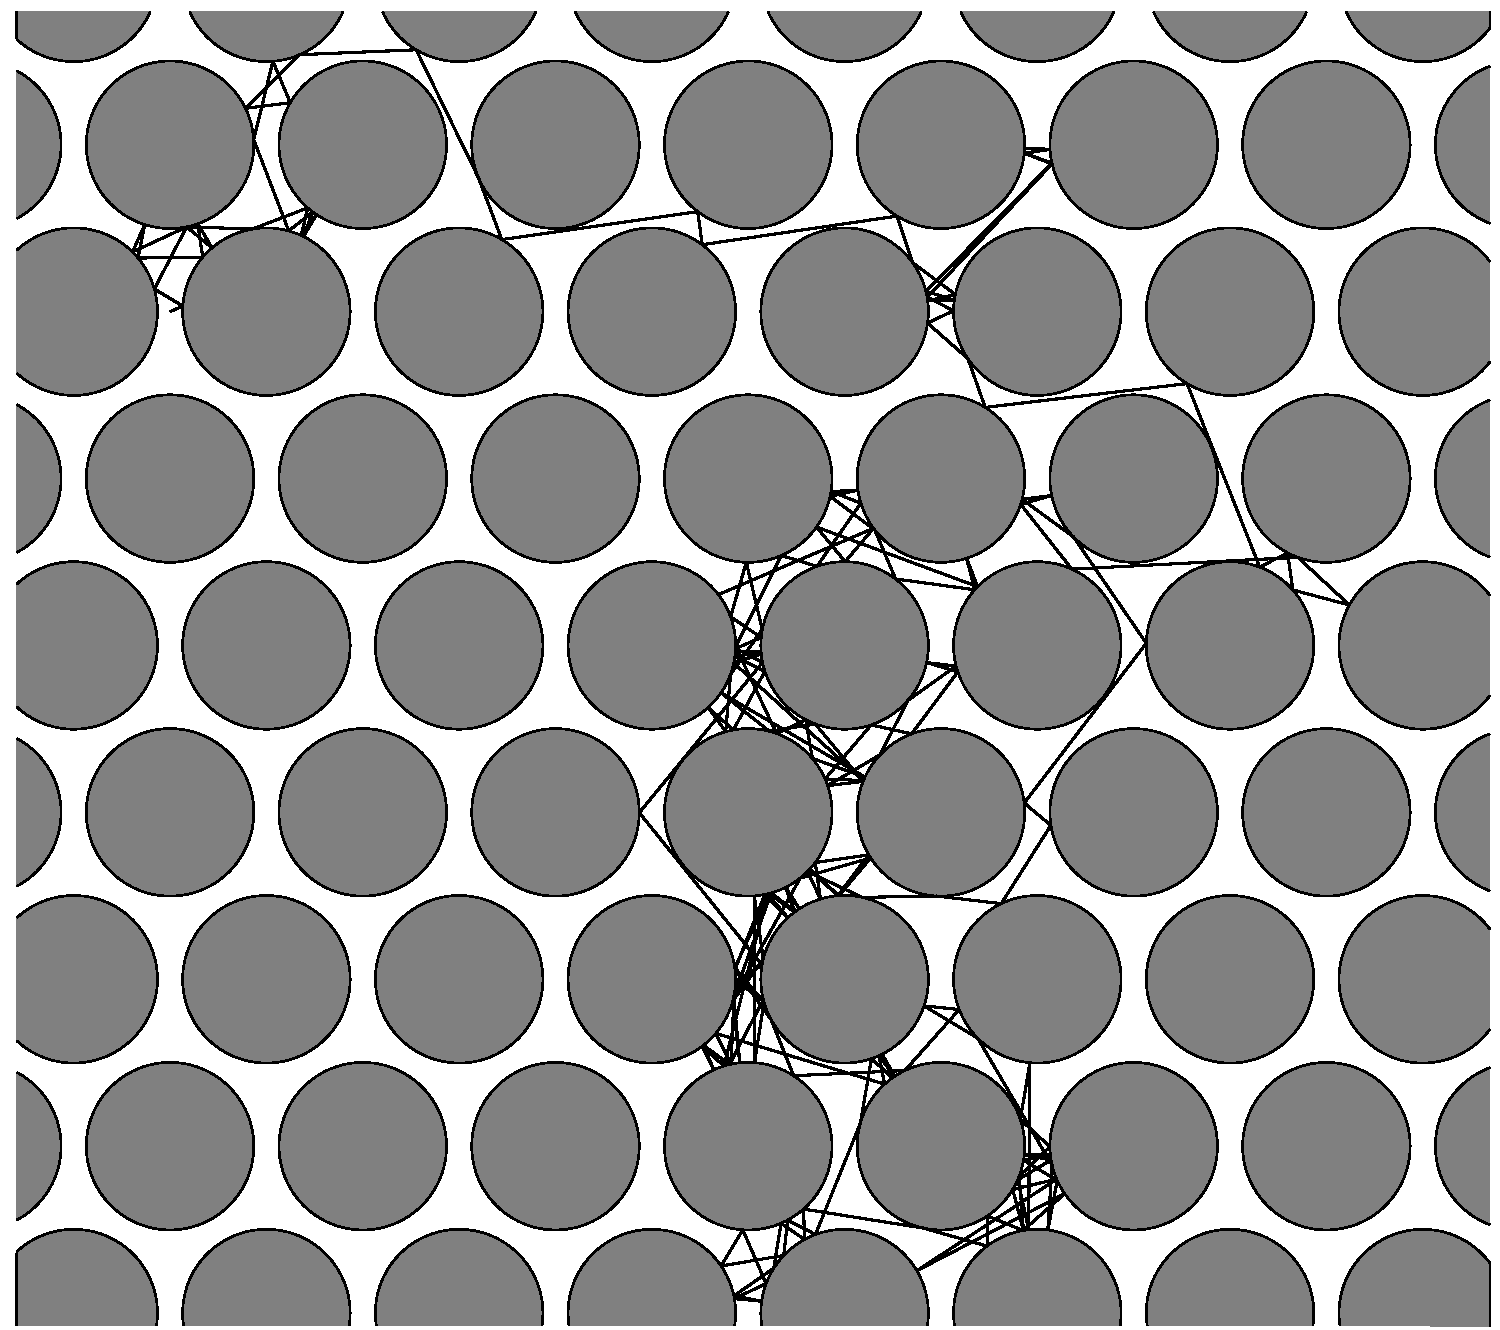
\includegraphics[width=0.45\textwidth]{diffuseChaoticBouncing}
    (b)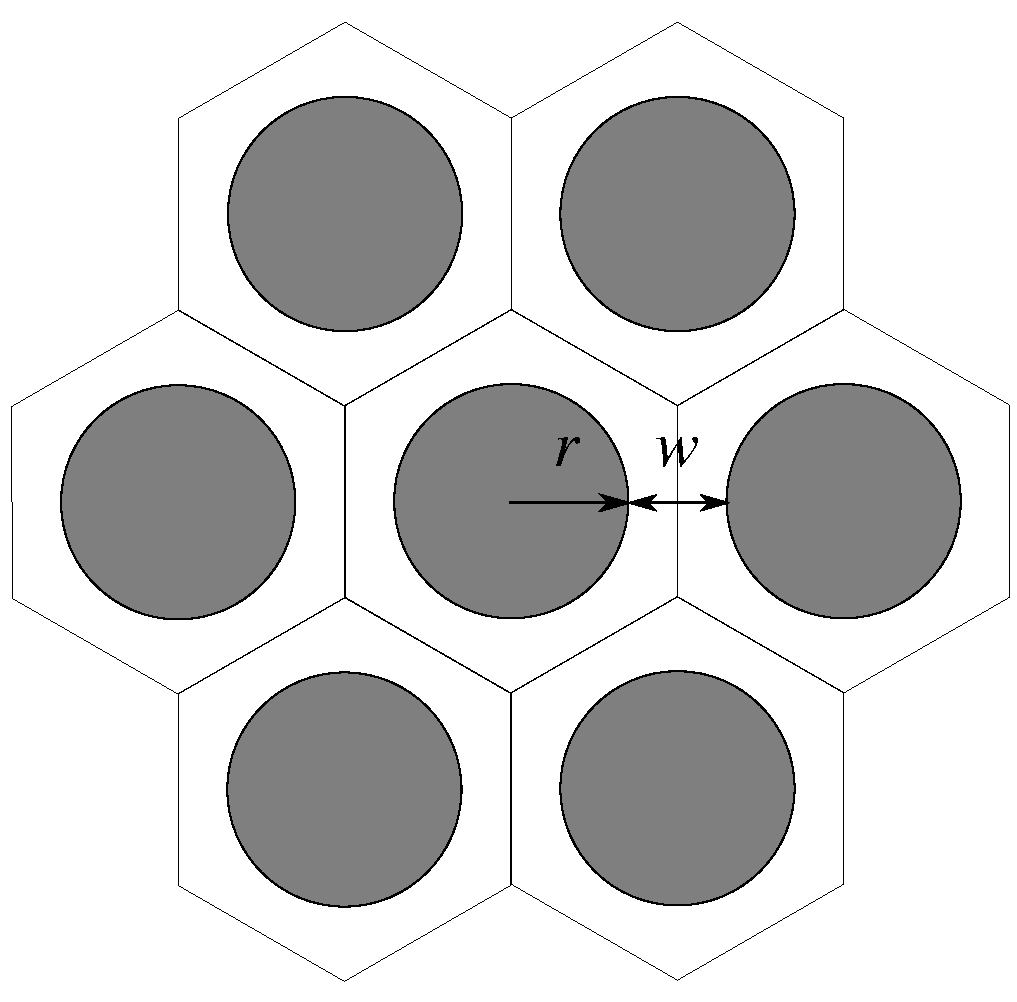
\includegraphics[width=0.45\textwidth]{diffuseLorentzGasParams}
  \end{center}
  \caption[]{\label{fig-chaoticBouncing}
  Motion in the Lorentz gas system. (a)  The chaotic trajectory of a
  ``gas'' particle bouncing in the array of disks  arranged in a
  hexagonal lattice pattern. The distance between disks are close  enough
  such that the particle has no infinite free flight (finite horizon).
  (b) A portion of the triangular Lorentz gas    system. The ratio of
  distance $w$ between the nearest pair of disks to the    disk radius
  $r$ determines the dynamical properties in the system.
  }
\end{figure}


\bigskip
=========== TO REUSE ========

    \PC{edits based Cvitanovi\'c,  Eckmann,and Gaspard\rf{LorentzDiff}}
The lattice symmetry of the Lorentz billiard has important consequence on
the properties of the function $Q(\beta)$ are best illustrated by
introducing its analytic continuation at $\beta = i k$.  The function
$F(k)=Q(ik)$ is the rate associated with the incoherent scattering
function $\langle \exp i k \cdot (\hat x_t - x) \rangle_M$ considered in
light or neutron scattering experiments in liquids, in particular, by Van
Hove\rf{BoonYip80,VanHove54}. The vector $k$ is interpreted as the
wavenumber of the hydrodynamic modes of diffusion which we also find in
the Lorentz gas.  The function $F(k)$ turns out to be a dispersion
relation since $F(k)=-D k^2 + {\cal O}(k^4)$ in an isotropic diffusive
system.  The isotropy of a liquid implies that the dispersion relation
only depends on the amplitude $\vert k\vert$ of the wavenumber.


On the other hand, the lattice symmetry of the Lorentz gas
imposes special restrictions on the properties of the dispersion relation
$F(k)$ and on the values taken by the wavenumber.  The present classical
problem of diffusion is similar to the quantum motion of a particle in a
periodic potential.  Hence, the wavenumber takes its values in the so-called
Brillouin zone\rf{BoSmWi36,Harrison70}.  A mode of diffusion is associated with each value of
the wavenumber $k$ so that the direction of $k$ is privileged in the
system.  As a consequence, the symmetry of the lattice is reduced by the choice
of $k$.  This symmetry reduction is formalized by the concept of little group
associated with the wavenumber $k$, which is the subgroup of the lattice point
group leaving invariant the vector $k$.  For most values of $k$ inside the
Brillouin zone, the little group is trivial because it contains only the
identity.  However, the little group is larger when the wavenumber belongs to
special symmetry lines or symmetry points in the Brillouin zone.  In particular,
the little group coincides with the full point group when $k=0$.

The preceding considerations concern the consequences of the lattice symmetry
on the factorization of the zeta function.  There is a different problem which
is to express the zeta function in terms of the prime periodic orbits of the
fundamental domain $\tilde M$ of the lattice (see Fig. 2) rather than
those of the elementary (Wigner-Seitz) cell $M$.
%This problem is a priori independent of the factorization
%discussed above and presents the following difficulty.
Here the stumbling block appears to be
the breaking of the rotational symmetry by
the auxilliary vector $\beta$, or, in other words,
the non-commutativity of translations and rotations.
More precisely, the global distance
$ \hat\phi^{r \period{\tilde{p}}} (\tx{\tpk}) - \tx{\tpk} $, $\tx{\tpk} \in \tp$,
% $ \hn_{r |\t p|}(\tx{\tpk}) $
depends on the starting cycle point if
$\tp$ is only a segment of the global cycle $p$. An
example is the diamond-shaped cycle of Fig.~3;
%the problem is that the $\tp$ segment of
%the global trajectory is not a translation in $\hM$.
depending whether one starts at $\tx_1$ or $\tx_2$, the global
distance covered in time $\period{\tilde{p}}$ is either the short or the
long diagonal.

In triangular and square lattices the diffusion is isotropic, but the
full function $Q(\beta)$ contains more information on the lattice
symmetry than the diffusion matrix of the second derivatives of
$Q(\beta)$. The behavior of the function $Q(\beta_x, \beta_y)$ away from
$\beta=0$ is discussed in \refref{Gaspard92a}. \PC{2015-12-03}{Lattice
gases literature (Hasslacher, Frisch?) has a reference to a formula in
Landau-Lifshitz that shows triangular lattice is isotropic - try to
re-find this.}

Compared to earlier literature\rf{CvitaEckardt,robb}, the new feature of the
problem at hand is use of vector-valued functions. The arbitrary vector
$\beta$ is only a device for generating moments~--~the moments themselves
are invariant under discrete symmetries, but it can be interpreted in
terms of the wavenumber of the hydrodynamic modes of diffusion.

The stumbling block
appears to be
 the breaking of the rotational symmetry by
 the auxilliary vector $\beta$, or, in other words,
the non-commutativity of translations and rotations.
More precisely,
in contrast to Eq.~(11), the global distance
$ \hf^{r \period{\tilde{p}}} (\tx{\tpk}) - \tx{\tpk} $, $\tx{\tpk} \in \tp$,
 $ \hn_{r |\t p|}(\tx{\tpk}) $
depends on the starting cycle point if
$\tp$ is only a segment of the global cycle $p$. An
example is the diamond-shaped cycle of Fig.~3;
the problem is that the $\tp$ segment of
the global trajectory is not a translation in $\hM$.
depending whether one starts at $\tx_1$ or $\tx_2$, the global
distance covered in time $\period{\tilde{p}}$ is either the short or the
long diagonal. We have not found a natural way of associating
a global distance in  formula Eq.~(17) with a fundamental domain
cycle $\tp$.

    \PC{the text from Cvitanovi\'c, Gaspard and Schreiber\rf{CGS92}}
In the periodic Lorentz gas\rf{Lorentz1905}
a point particle reflects elastically off
a periodic array of reflecting disks in a plane.
The system can
be thought of as an unfolding of the Sinai billiard\rf{Sinai70}.
The standard diffusion constant can be defined if the particle has a bounded
free path between any two successive bounces.
An example is a triangular array with sufficiently small
inter-disk spacing.
Unfortunately, as we shall see,
the same mechanism that guarantees a finite horizon
also leads to rather awkward pruning of periodic orbits.

    \PC{edits based Cvitanovi\'c,  Eckmann,and Gaspard\rf{LorentzDiff}}
In \refrefs{art91,LorentzDiff,CGS92,Artuso94,CBdiffusion}  an explicit
connection between the global diffusion and the dynamics restricted to
an elementary cell.
Our method applies to any  hyperbolic dynamical system that is
a periodic tiling $\hM=\bigcup_{ \hn \in T} M_{
\hn}$
of the dynamical phase space $\hM$ by {\sl translates}
$M_{\hn}$
of an {\sl elementary cell} $M$, with $T$ the abelian group of lattice
translations.
Furthermore, each elementary cell may be built from a
{\sl fundamental domain}
$\tM$
by the action of a discrete (not necessarily Abelian) group $G$.

                                                            \toCB
Generalization to continuous time\rf{bowen,pexp} amounts to the replacement
%$ z\,=\,e^{-s} $,
$ z^{\period{p}} \rightarrow e^{-s \period{p}} $,
where $\period{p}$ is now the (not necessarily integer)
%{\sl time-}
period of the prime cycle $p$:
$$
Z(\beta,s)\,=\,\prod_{p\in\PP} \exp \left( - {
 \sum_{r=1}^\infty {1 \over r}
 { e^{(\beta \cdot \hn_p- s \period{p}) r } % z^{n_p r}
 \over { | \det \left( {\bf 1}-{\bf J}_p^{r} \right) | } }
 } \right)
\,\, .
%Eq.~(14)
$$


 As we are concerned with the long time behavior,
 this problem can be circumvented
 by replacing $ \hf^t(\tx{\tpk}) $ by the mean
 drift in the $t \rightarrow \infty$ limit.
 $ \hf^t(\tx{\tpk}) $ is a translation in $\hM$ for each
 complete cycle $p$ in $M$, so we replace
 \bea
 \hf^t(\tx{\tpk}) - \tx{\tpk}
 \,\Longrightarrow \,
 &&
 { { \hf^{m_p t}(\tx{\tpk}) - \tx{\tpk} }
 % \over         m_p
 }
    % \,\equiv \, r {\tilde n}_{\tp} (\tx{\tpk})
 \continue
t &=& r \period{\tilde{p}}, \quad m_p = \period{p}/\period{\tilde{p}} \quad \tx \in \tp \,\, ,
 \eea
 in Eq.~(240).
 The magnitude of ${\tilde n}_{\tp}(\tx{\tpk})$, the mean
 global drift per one traversal of the fundamental cycle $\tp$, is
 independent of the starting point, but its direction is not; the
 reason is that each fundamental domain cycle corresponds to a set of
 trajectories in $\hM$.
 The ${1 \over {|G|}} \sum$ average in
 Eq.~(240) then generates all distinct global drift
 directions, so we can again replace the
 sum over cycle points by the factor $\period{\tilde{p}}$, and obtain the
 $Z$ function Eq.~(14) for the $\alpha $ irreducible subspace
 $$
 Z(\beta,s)_\alpha\,=\,\prod_{\tp \in \t{\cal{P}} } \exp
 % \left( -
  % \sum_{r=1}^\infty {1 \over r}
 % {{
  % \chi_\alpha(h^r_{\tp})
  % }
 % \over
 % { | \det \left( \bf{1}-\t{\bf J}_{\tp}^{r} \right) | }
 % }
 % e^{ ( \beta \cdot {\tilde n}_{\tp} - s \period{\tilde{p}}) r}
  % \right)
 \,\, .
 Eq.~(24)
 $$
 $\hn_{\period{\tilde{p}}}(\tx_k)$
%{\tt NOnsense...}
 The leading eigenvalue of the
unsymmetrized
 operator Eq.~(8) is
 the leading eigenvalue of the symmetric subspace for which
 $\chi_\alpha(g)=1$ for all $g \in G$.




Machta and Zwanzig\rf{MacZwa83} have given numerical results
for the diffusion constant in Lorentz gases,  as well as
estimates based on a random walk approximation. We shall follow
their notation and fix the radius of the disks to 1,
assume unit particle speed, and
denote the spacing between the disks by $w$ (see fig.~1).
The horizon is finite for $w < 4/\sqrt{3}-2 = 0.3094\dots$.


\subsection{Periodic orbit theory}
\label{s-POT}
  % POT.tex      pdflatex ZhCvGo15
% Diffuse globally, compute locally: a cyclist tale
% Tingnan Zhang, Daniel I. Goldman and Predrag Cvitanovi\'c

% \subsection{Periodic orbit theory}
% \label{s-POT}

\Po\ theory of deterministic diffusion, introduced in
\refrefs{art91,LorentzDiff}, exploits the fact that the periodic Lorentz
gas can be constructed by putting together translated copies of an
elementary cell. Therefore quantities characterizing global dynamics,
such as the Lyapunov exponents and the diffusion tensor, can be computed
from the dynamics restricted to the elementary cell, as shown numerically
in \refref{CGS92}.

In \refrefs{art91,LorentzDiff,CGS92,Artuso94,CBdiffusion} it was shown that
deterministic diffusion tensor in the {\em periodic} Lorentz gas can be
expressed in terms of (relative) \po s, and exact \cycForm\ for such
global dynamical averages as Lyapunov exponent and diffusion tensor were
derived, using only the dynamics in the elementary cell. For any
dynamical system that has translational symmetry,the full state space
$\hM$ (i.e., both spatial coordinates and momenta) has aperiodic tiling
\[ %beq
\hM=\bigcup_{ \hn \in T} \pS_{\hn},
\] %eeq
by {\em translating} $\pS_{\hn}$ of an {\em elementary cell} $\pS$, with
$T$ the abelian group of lattice translations.

In the context of Lorentz gas system, the elementary cell is the
hexagonal region centered at the scatterer, see
\reffig{fig-chaoticBouncing}\,(a). The dynamics restricted inside the
elementary cell is understood as the periodic boundary condition: when
the particle leaves the edge of the hexagon cell, it immediately enters
the region again from the opposite edge. We distinguish two types of
diffusive behavior; the {\em infinite horizon} case, which allows for
infinite length flights, and the {\em finite horizon} case, where any
free particle trajectory must hit a disk in finite time. The transition
between horizon and infinite horizon is controlled by the ratio of $w/r$,
where $w$ is the gap between nearest pair of disk and $r$ the radius of
the disk.

    \PC{2013-02-03}
    { Roberto says we must
incorporate kneading determinants from
Cristadoro\rf{ArtCri03,Cristad06,CriKnDeEsp12}.
    }


    \PC{2015-10-21}
    {edits based Cvitanovi\'c,  Eckmann,and Gaspard\rf{LorentzDiff}}
In \refrefs{art91,LorentzDiff,CGS92,Artuso94,CBdiffusion}  an explicit
connection between the global diffusion and the dynamics restricted to
an elementary cell.
Our method applies to any  hyperbolic dynamical system that is
a periodic tiling $\hM=\bigcup_{ \hn \in T} M_{
\hn}$
of the dynamical phase space $\hM$ by {\sl translates}
$M_{\hn}$
of an {\sl elementary cell} $M$, with $T$ the abelian group of lattice
translations.
Furthermore, each elementary cell may be built from a
{\sl fundamental domain}
$\tM$
by the action of a discrete (not necessarily Abelian) group $G$.

                                                            \toCB
Generalization to continuous time\rf{bowen,pexp} amounts to the replacement
%$ z\,=\,e^{-s} $,
$ z^{\period{p}} \rightarrow e^{-s \period{p}} $,
where $\period{p}$ is now the (not necessarily integer)
%{\sl time-}
period of the prime cycle $p$:
$$
Z(\beta,s)\,=\,\prod_{p\in\PP} \exp \left( - {
 \sum_{r=1}^\infty {1 \over r}
 { e^{(\beta \cdot \hn_p- s \period{p}) r } % z^{n_p r}
 \over { | \det \left( {\bf 1}-{\bf J}_p^{r} \right) | } }
 } \right)
\,\, .
%Eq.~(14)
$$


 As we are concerned with the long time behavior,
 this problem can be circumvented
 by replacing $ \hf^t(\tx{\tpk}) $ by the mean
 drift in the $t \rightarrow \infty$ limit.
 $ \hf^t(\tx{\tpk}) $ is a translation in $\hM$ for each
 complete cycle $p$ in $M$, so we replace
 \bea
 \hf^t(\tx{\tpk}) - \tx{\tpk}
 \,\Longrightarrow \,
 &&
 { { \hf^{m_p t}(\tx{\tpk}) - \tx{\tpk} }
 % \over         m_p
 }
    % \,\equiv \, r {\tilde n}_{\tp} (\tx{\tpk})
 \continue
t &=& r \period{\tilde{p}}, \quad m_p = \period{p}/\period{\tilde{p}} \quad \tx \in \tp \,\, ,
 \eea
 in Eq.~(240).
 The magnitude of ${\tilde n}_{\tp}(\tx{\tpk})$, the mean
 global drift per one traversal of the fundamental cycle $\tp$, is
 independent of the starting point, but its direction is not; the
 reason is that each fundamental domain cycle corresponds to a set of
 trajectories in $\hM$.
 The ${1 \over {|G|}} \sum$ average in
 Eq.~(240) then generates all distinct global drift
 directions, so we can again replace the
 sum over cycle points by the factor $\period{\tilde{p}}$, and obtain the
 $Z$ function Eq.~(14) for the $\alpha $ irreducible subspace
 $$
 Z(\beta,s)_\alpha\,=\,\prod_{\tp \in \t{\cal{P}} } \exp
 % \left( -
  % \sum_{r=1}^\infty {1 \over r}
 % {{
  % \chi_\alpha(h^r_{\tp})
  % }
 % \over
 % { | \det \left( \bf{1}-\t{\bf J}_{\tp}^{r} \right) | }
 % }
 % e^{ ( \beta \cdot {\tilde n}_{\tp} - s \period{\tilde{p}}) r}
  % \right)
 \,\, .
 Eq.~(24)
 $$
 $\hn_{\period{\tilde{p}}}(\tx_k)$
%{\tt NOnsense...}
 The leading eigenvalue of the
unsymmetrized
 operator Eq.~(8) is
 the leading eigenvalue of the symmetric subspace for which
 $\chi_\alpha(g)=1$ for all $g \in G$.


Machta and Zwanzig\rf{MacZwa83} have given numerical results
for the diffusion constant in Lorentz gases,  as well as
estimates based on a random walk approximation. We shall follow
their notation and fix the radius of the disks to 1,
assume unit particle speed, and
denote the spacing between the disks by $w$ (see fig.~1).
The horizon is finite for $w < 4/\sqrt{3}-2 = 0.3094\dots$.

We now relate the dynamics in $\pS$ to diffusive properties of the
Lorentz gas in $\hM$. Let $\hx(t)\,=\,\hflow{t}{\hx_0}$ denotes the point
in the global space $\hM$ reached by the flow in time $t$.
$x(t)\,=\,\flow{t}{\xInit}$ denotes the corresponding flow in the
elementary cell; the two are related by
\beq
\hn_t(\xInit)=\hflow{t}{\xInit} - \flow{t}{\xInit} \in T \,,
\ee{l-diff-hatn1}
the translation of the endpoint of the global path into the elementary cell $\pS$.

Fix a vector $\beta \in \reals^d$, where $d$ is the dimension of
the{\statesp}. We will compute the diffusive properties of the Lorentz
gas from the leading eigenvalue of the Rulle-Frobenius-Perron \evOper\
\beq
\eigenvL(\beta)\,=\, \lim_{t \rightarrow \infty} \frac{1}{t} \log \langle
e^{\beta \cdot (\hx(t) -x) } \rangle_\pS ~, \quad
\label{eq-diff-1}
\eeq
where the average is over all initial points in the elementary cell, $x
\in\pS$. If all odd derivatives vanish by symmetry, there is no drift and
the second derivatives
\begin{widetext}
\beq
2d D_{ij} = \left . {\frac{\partial}{\partial \beta_i}} {\frac{\partial}
{\partial \beta_j}} \eigenvL(\beta)\right\vert_{\beta=0} \,=\,\lim_{t\rightarrow
\infty} {\frac{1}{t}} \langle {(\hx(t) -x)_i (\hx(t) -x)_j } \rangle_\pS ~,
\eeq
\end{widetext}
yield a diffusion matrix.  This symmetric matrix can, in general, be
anisotropic(\ie, have $d$ distinct eigenvalues and eigen\-vectors). The
spatial diffusion constant is then given by the Einstein relation
\beq
D\,=\,{1\over 2 d} \sum_i \left .{{\partial}^2 \over {\partial
      \beta^2_i}} \eigenvL(\beta)\right |_{\beta=0} \,=\,
\lim_{t\rightarrow \infty} {1\over{2d t}} \langle {(\hat{q}(t) -q)^2 }
\rangle_\pS~ ~,
\eeq
where the $i$ sum is restricted to the spatial components $q_i$ of
the{\statesp} vectors $x=(q,p)$, \ie, if the dynamics is Hamiltonian, the
sum is over the $d$ degrees of freedom.
\PC{2014-11-18}{reinstate mass, velocity, size to get $\beta$, $m$, $\sigma$
    dependencies right?}

We now turn to the connection between diffusion and periodic orbits in
the elementary cell. It was shown in \refref{CGS92} that the ensemble
average in\refeq{eq-diff-1} can be written as an integral over the
elementary cell
\beq
\langle e^{\beta\cdot(\hx(t)-x)} \rangle
   = \frac{1}{\vert \pS \vert}\int_{x,y\in \pS} dxdy {\cal L}^t(y,x),
\eeq
given the linear \evOper
\beq
{\cal L}^t(y,x) = e^{\beta\cdot(\hx(t)-x)}\delta(y-x(t))
\label{eq-eOper}
\eeq
The interesting dynamical averages is determined by the spectrum of the operator
\beq \det(\eigenvL - \Lop) \,=\,\prod_{p} \exp \left(
  - { \sum_{r=1}^\infty {1 \over r} { e^{(\beta \cdot \hn_p- s
        \period{p}) r} \over \oneMinJ{r} }
  } \right) \,,
\ee{lor-diff-14}
or the corresponding \dzeta\
\beq
1/\zeta(\beta, s)\,=\,\prod_{p}\left( 1 - \frac{e^{(\beta \cdot \hn_p-
      s \period{p})}}{|\ExpaEig_p|} \right) ~,
\label{zeta-diff}
\eeq
where $\period{p}$ is the period of the cycle and $\ExpaEig_p$ the
product of expanding eigenvalues of the cycle\rf{DasBuch}.

The \dzeta\ \cycForm\ for the diffusion constant, zero mean drift
$ \expct{ \hat{x}_i } = 0 \,, $ is given by
 \beq D \,=\,{1 \over 2 d}
{ \expct{\hat{x}^2}_\zeta \over \expct{\period{}}_\zeta } \,=\,{1
  \over 2 d } \, {1 \over \expct{\period{}}_\zeta} \sumprime
\frac{(-1)^{k+1} (\hn_{p_1}+ \cdots+ \hn_{p_k})^2}
{|\ExpaEig_{p_1}\cdots \ExpaEig_{p_k}|} \, ,
\label{eq-ecDiffCoef}
\eeq
where the sum is over all distinct non-repeating combination of prime
cycles (in the elementary cell). The derivation is standard, still the
formula is strange.Diffusion is unbounded motion across an infinite
lattice; nevertheless, the reduction to the elementary cell enables us to
compute relevant quantities in the usual way, in terms of periodic
orbits.


%\section{Into the fundamental domain}
%\label{s-SymmetryReduction}

\section{Into the fundamental domain}
\label{s-SymmetryReduction}
\begin{figure}[htbp]
  \begin{center}
    (a)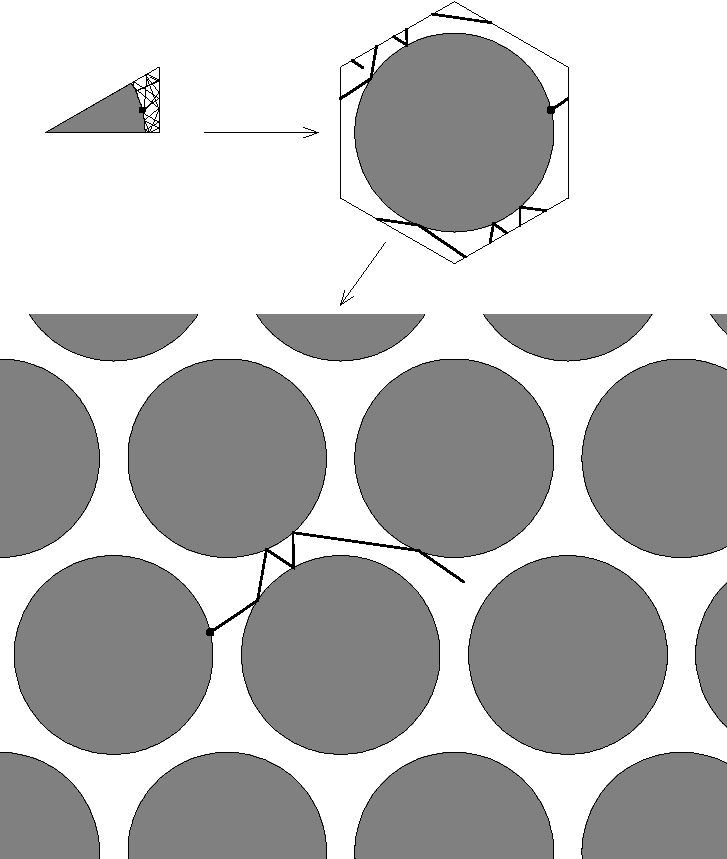
\includegraphics[width=0.45\textwidth]{diffuseSchreiberFig1}
    (b)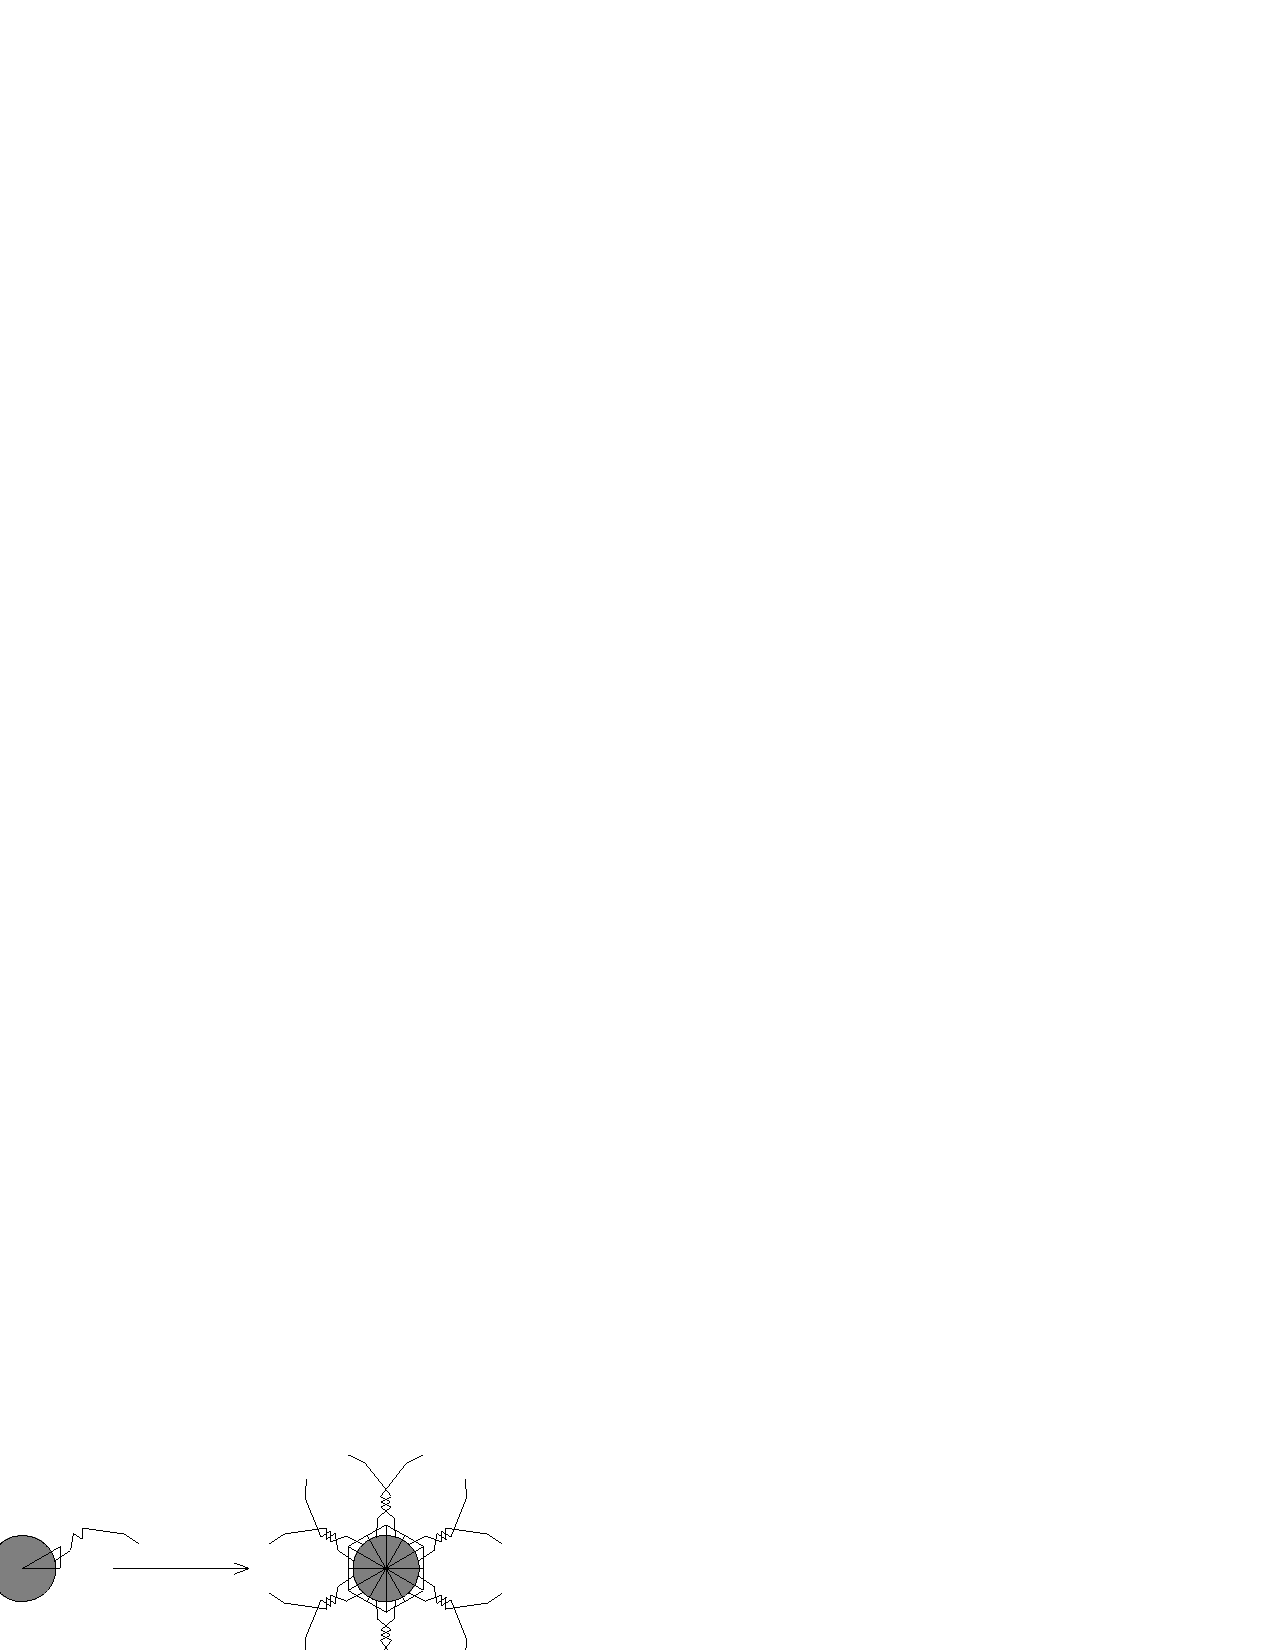
\includegraphics[width=0.45\textwidth]{diffuseSchreiberFig2}
  \end{center}
  \caption[]{\label{fig-schrieberFig12}
  (a) Motion in the fundamental domain (top left), elementary cell (top
      right) and  in full space (bottom).
  (b) An (unwrapped) trajectory (in full  space) and its 12 copies after
      applying point group actions to it.
  }
\end{figure}

%\begin{figure}[htbp]
%  \begin{center}
%    (a)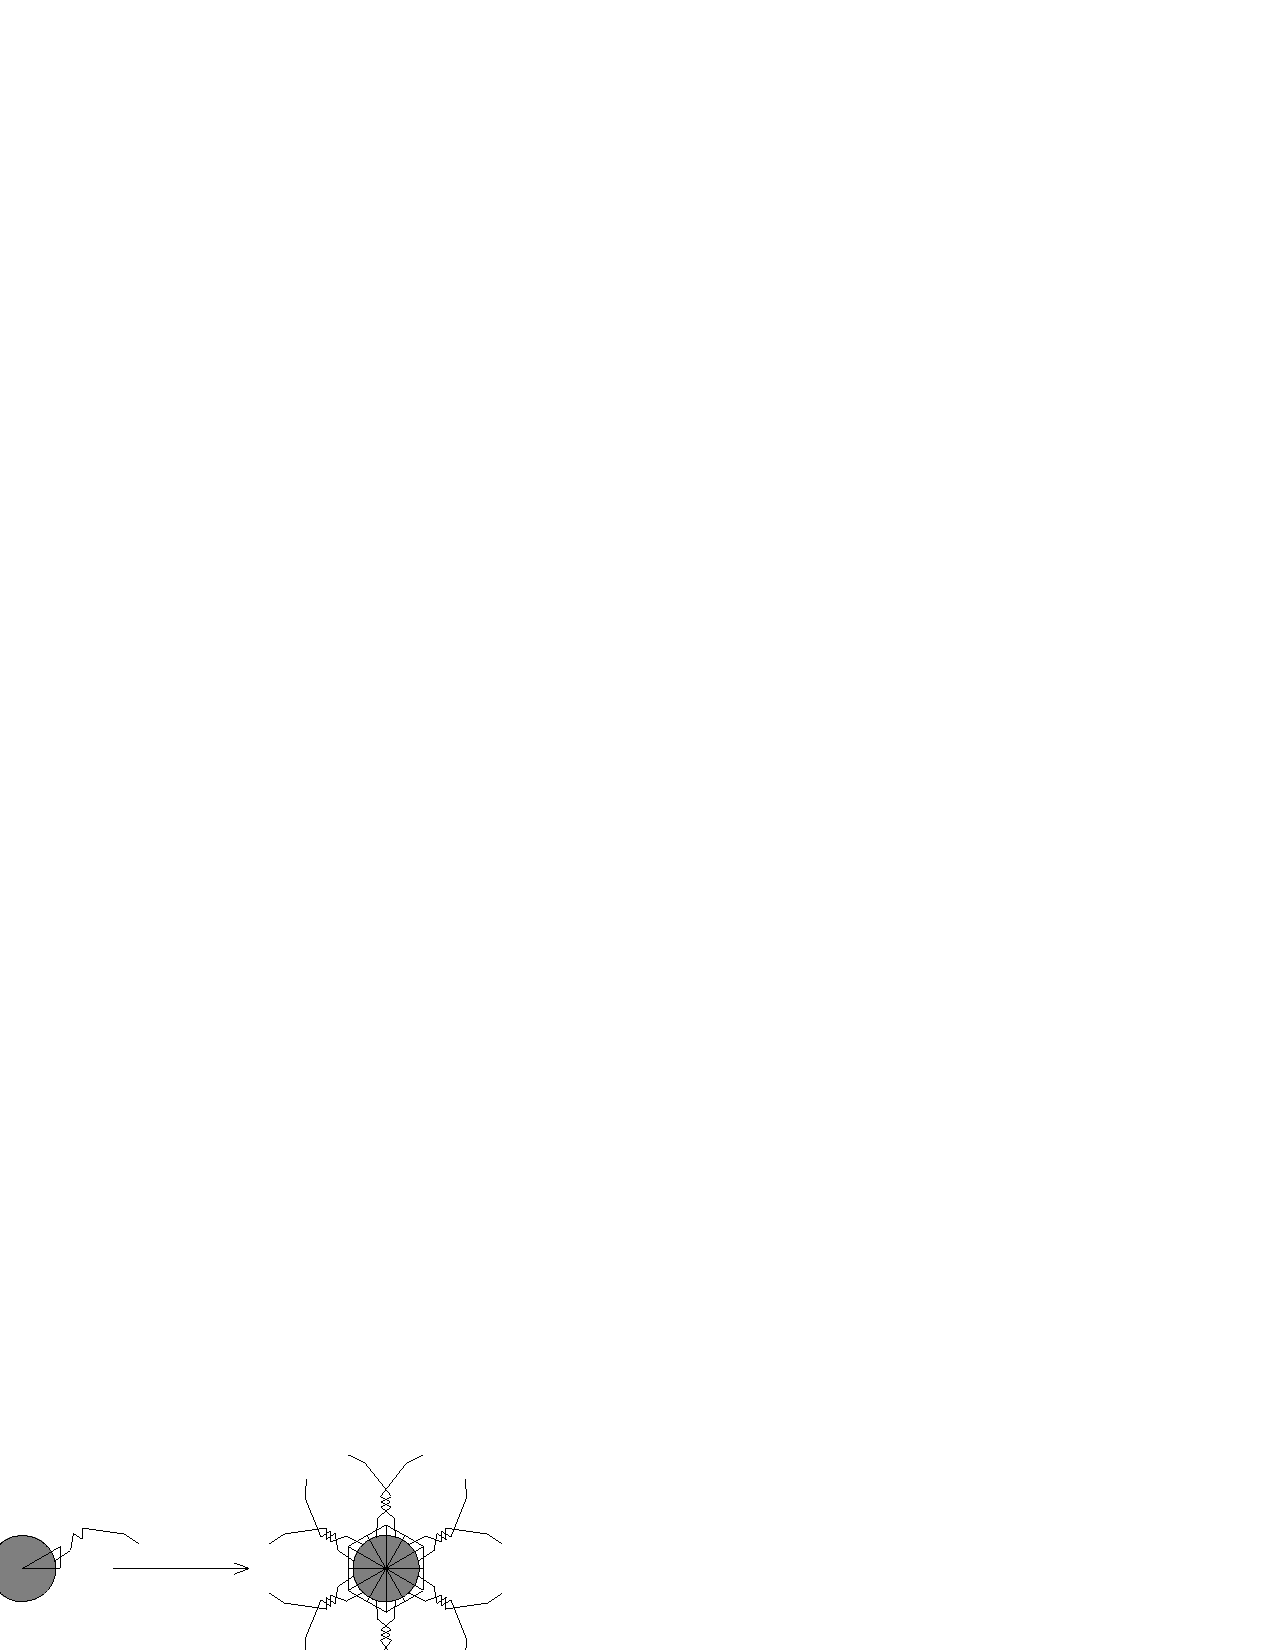
\includegraphics[width=0.45\textwidth]{diffuseSchreiberFig2}
%    (b)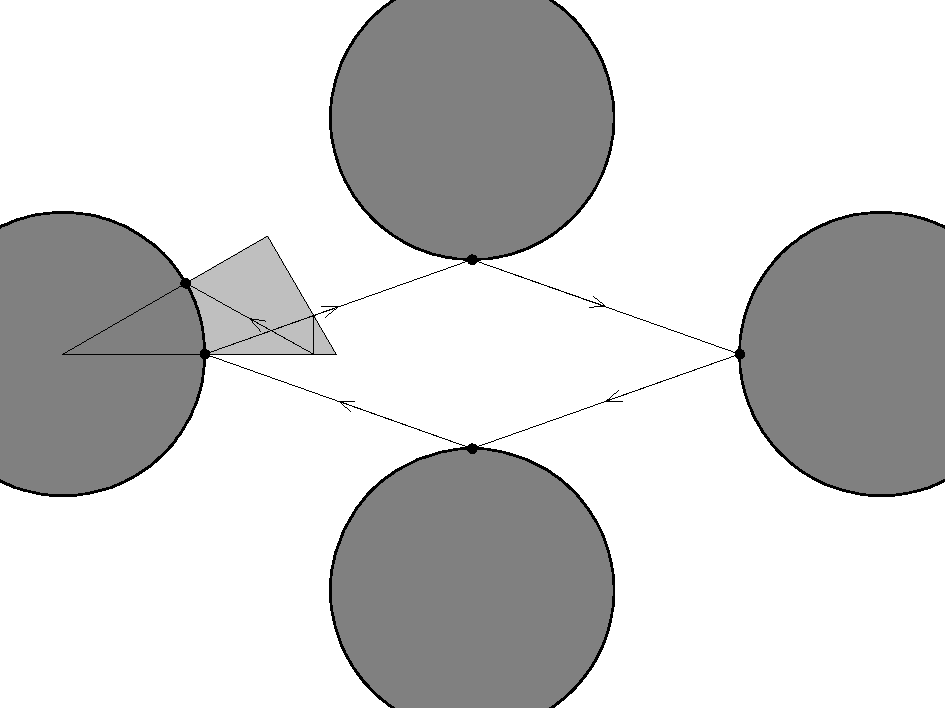
\includegraphics[width=0.45\textwidth]{diffuseSchreiberFig3}
%  \end{center}
%  \caption[]{ \label{fig:schrieberFig23} (a) An (unwrapped) trajectory (in full
%  space) and its 12 copies after applying point group actions to it. (b)
%  Multiplicity of periodic orbits in fundamental domain.}
%\end{figure}

When the scattering array has further discrete symmetries, such as
reflection symmetry, each elementary cell may be built from a {\em
fundamental domain} ${\widetilde \pS}$ by the action of a discrete (not
necessarily abelian) group $G$. The quantity $\tx(t)\,=\,\tflow{t}{\tx}$
denotes the flow in the fundamental domain ${\widetilde \pS}$;
$\tflow{t}{\tx}$ is related to$\flow{}{\tx}$ by a discrete symmetry $g
\in G$ which maps $\tx(t)\in{\widetilde \pS}$ to ${x}(t) \in {\pS}$. The
full $\hM \rightarrow {\widetilde\pS}$ reduction is complicated by the
non-abelian nature of $G$, and will be illustrated in this section in
detail.

\subsection{How point group changes translation}

In the fundamental domain, one has to realize a few facts before
proceeding to the cycle expansion derivation. A point $x$ in the
elementary cell can be uniquely identified by its ``mirror image'' in the
fundamental domain:
\[ %beq
x=g\circ\tx,
\] %eeq
given a group action $g\in G$ the discrete symmetry group. In the
triangular periodic Lorentz gas the underlying point group is $C_{6v}$
(isomorphic to $D_6$), and the hexagonal elementary cell is partitioned
into 12 identical triangular domains. We have to appreciate that the flow
$\hat{\phi}^t$ is G-equivariant under the lattice group symmetry, and
proceed with the argument that the displacement in full space is also
equivariant under the point group symmetry (which is a subset of the
lattice group):
\[ %beq
\hn_t(x)\equiv\hn_t(g\circ\tx)= g\circ\hn_t(\tx).
\] %eeq

We can apply this fact to the displacement associated with a prime
periodic orbit $\tp$ restricted in the fundamental domain.
Let$\tp\equiv\{\tx_0,\tx_1,\ldots,\tx_{N_\tp}\}$, with topological length
$N_\tp$and $\tx_i$ the bouncing points on the orbit. For each flight
(e.g. from $\tx_i$to $\tx_{i+1}$) we denote the associated displacement
in full space $\hn(\tx_i,e)$. However, one has to be careful when adding
the individual displacements together when moving along a fundamental
domain orbit. Unlike in elementary cell, the fundamental domain point
$\tx_i$ does not distinguish in which triangular piece it is. Instead, we
assign a point group element$g_\tp(\tx_{i+1},\tx_{i})$ to keep track of
changes in absolute orientation. We now write the displacement traveled
along the orbit, after finishing a full cycle:
\beq
\hn_{\tp}(\tx_{0})=\sum_{i=0}^{N_\tp-1}\hn(\tx_{i},g_{\tp,\tx_0}(\tx_{i}))=\sum_{i=0}^{N_\tp-1}g_{\tp,\tx_{0}}(\tx_{i})\circ\hn(\tx_{i},e),
\eeq
where $g_{\tp,\tx_{0}}(\tx_i)=\prod_0^{j-1} g_\tp(\tx_{j+1},\tx_{j})$ is
the accumulated orientation changes along the orbit when starting from
$\tx_{0}$.The displacement now has its dependence on the starting point
we choose. We denote the total group action for the orbit

\bea
h_{\tp}(\tx_i)&\equiv& g_\tp(\tx_{i},\tx_{i-1})\circ\ldots\circ
g_\tp(\tx_{0},\tx_{N_\tp-1})\nonumber\\
&& \circ g_\tp(\tx_{N_\tp-1},\tx_{N_\tp-2})\circ \ldots\circ
g_\tp(\tx_{i+1},\tx_{i}),
\eea
which one can immediately see the connection
$\flow{t_\tp}{\tx_i}=h_{\tp}(\tx_i)\tflow{t_\tp}{\tx_i}$.
Although the group action $h_{\tp}(\tx_i)$ depends on the initial points
on the orbit, it is a property of the orbit's symmetry, and subsequently
all $h_{\tp}(\tx_i), \tx_i\in\tp$ belong to the \emph{same} subgroup of
$G$.

We define the quantity:
\beq
\hat{L}_{\tp}^{r}(\tx_i)\equiv
(e+\hp^{1}(\tx_i)+\cdots+\hp^{r-1}(\tx_i))\cdot\hn_{\tp}(\tx_i),
\label{eq-fdDisplacement}
\eeq
to be the displacement traveled along the orbit $r$ times, starting from
$\tx_i$.  Though one may not appreciate immediately,
\refeq{eq-fdDisplacement} takes care of the rotational symmetry that does
not commute with translation, and we will show that it gives the proper
displacement needed for computing diffusion coefficient in the
fundamental domain.


\subsection{Gymnastics of equations}

We properly treat the discrete symmetry by projecting the trace of\evOper
\refeq{eq-eOper} to the group's subspace:
 \bea
\tr{\cal L}^t &=& \sum_{\alpha \in\II_G} \tr{\cal L}_{\alpha}^t\nonumber\\
\tr{\cal L}_{\alpha}^{t} &=& \frac{d_\alpha}{|G|}\sum_{\sigma \in
  G}\sum_{h\in G}\chi_\alpha(h)\int_{\t {\cal M}} d\tx \delta (h\tx -
\flow{t}{\tx})e^{\beta\cdot\sigma\cdot\hn^t(\tx)}.\nonumber\\
\label{eq-traceSum}
\eea

The $\delta$-function part $\delta (h\tx - \flow{t}{\tx})$ in the integral
selects the fundamental domain periodic points that satisfy the group
condition $h\equiv h^r_{\tp}(\tx_i)$. The displacement traveled starting
from each of those points and along the orbit $r$ times takes the form
already computed in\refeq{eq-fdDisplacement}. The rest is straight
forward gymnastics of algebra,which yields the dynamical zeta function
for the $\alpha$ irreducible representation:
\begin{widetext}
 \beq
\frac{1}{\zeta_{\alpha}(\beta,s,z)}
=\exp\left(-\frac{d_\alpha}{|G|}\sum_{\sigma\in G}\sum_{\tp}
    \frac{1}{N_{\tp}}\sum_{\tx_{i}\in\tp}\sum_{r=1}^{\infty}
    \frac{t_{\tp}^{r}}{r}
    \chi_{\alpha}(\hp^{r}(\tx_i))e^{\beta\cdot\sigma\cdot\hat{L}_{\tp}(r,\tx_i)}
    \right),
\label{eq-fdZeta}
\eeq
\end{widetext}

where
\[
  t_{\tp}\equiv
\frac{z^{N_{\tp}}e^{-sT_{\tp}}}{|\ExpaEig_\tp|}
\,,
\]
is the weight associated to the orbit. Equation \refeq{eq-fdZeta}
differs from its counterpart in elementary cell, but can be reduced to if
the symmetry group contains only $e$.

We are interested in the one dimensional, symmetric trivial
representation with$ d_\alpha = 1 $ and all $ \chi(h) = 1 $; there by we
drop the subscript $\alpha $ in the following calculation. Partial
derivative with respect to$\beta$ gives:
\begin{widetext}
\bea
\frac{\partial^{2}}{\partial\beta^{2}}\frac{1}{\zeta(\beta,s,z)}
&=\frac{1}{\zeta(\beta,s,z)}\left(\left(\frac{1}{|G|} \sum_{\sigma\in G}\sum_{\tp}\sum_{\tx_i\in \tp}\sum_{r=1}^{\infty}\frac{\sigma\cdot \hat{L}_{\tp}^{r}(\tx_i)t_{\tp}^r e^{\beta\cdot\sigma\cdot \hat{L}_{\tp}^{r}(\tx_i)}}{N_{\tp}r}\right)^{2}\right.\nonumber\\
&\left.-\frac{1}{|G|}\sum_{\sigma\in G}\left(\sum_{\tp}\sum_{\tx_i\in
      \tp}\sum_{r=1}^{\infty}\frac{\vert \sigma\cdot
      \hat{L}_{\tp}^{r}(\tx_i)\vert^{2}t_{\tp}^{r}e^{\beta\cdot\sigma\cdot
        \hat{L}_{\tp}^{r}(\tx_i)}}{N_{\tp}r}\right)\right).
        \eea
\end{widetext}
The first term in the formula corresponds to $ \langle\hx\rangle^2 $ and
second to $ \langle\hx^2\rangle $. It is trivial to see that
\beq\sum_{\sigma\in G}\frac{\sigma\cdot
  \hat{L}_{\tp}^r(\tx_i)t_{\tp}^r e^{\beta\cdot\sigma\cdot
  \hat{L}_{\tp}(r,\tx_i)}}{N_{\tp}r} \equiv 0,
\eeq
because of the summation over the discrete group $G$. Thus the calculated
mean drift is zero, consistent with the symmetry of the system. Observing
that the length$\vert \sigma\cdot \hat{L}_{\tp}^{r}(\tx_i) \vert$ does
not change under rotation, we write
\bea
\langle\hx^2\rangle &=& \left.\frac{1}{\zeta(\beta,s,z)}\sum_{\tp}\sum_{r=1}^{\infty}\frac{t_{\tp}^{r}}{r}\sum_{\tx_i\in \tp}\frac{\vert\hat{L}_{\tp}^{r}(\tx_i)\vert^{2}}{N_{\tp}}\right\vert_{\beta=0,s=0, z=1} \nonumber\\
&=& \left.\prod_{\tp}\left(1-\frac{z^{N_{\tp}}}{\vert\ExpaEig_\tp\vert
    }\right)\sum_{\tp}\sum_{r=1}^{\infty}\left(\frac{z^{N_{\tp}}}{\vert\ExpaEig_\tp\vert
    }\right)^r\frac{\vert\hat{L}_{\tp}^{r}\vert^2}{r}\right\vert_{z=1}
\label{eq-meanSquareDisp}
\eea with $\hat{L}_{\tp}^{r}\equiv\sum_{\tx_i\in
  \tp}\frac{\vert\hat{L}_{\tp}^{r}(\tx_i)\vert^{2}}{N_{\tp}}$ the
average square displacement in full space when traveling along a fundamental domain $r$ times. Formula \refeq{eq-meanSquareDisp} is an infinite polynomial in the auxiliary variable $z$, and should be truncated to the topological length of the longest periodic orbits find in calculation.

\subsection{Grammar of fundamental domain cycle}

\begin{figure}[htbp]
  \begin{center}
    (a) 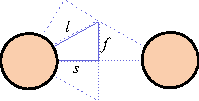
\includegraphics[width=0.35\textwidth]{diffuse7diskFundDflips}
    (b) 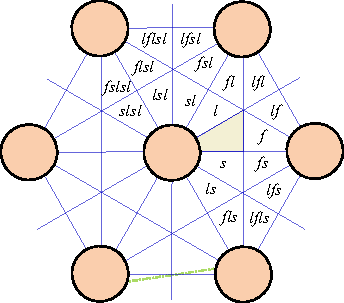
\includegraphics[width=0.35\textwidth]{diffuse7diskFundDtiles}
  \end{center}
  \caption{\label{fig-7diskFundDflips}
  (a) The three generators of tiling of the  plane by a fundamental
  domain: two generators of \Dn{12} tiling, reflection  $s$ across the
  short disk-disk separation, reflection $\ell$ across the long
  disk-disk separation; and a translation generator $f$ that pivots
  (`flips') a  disk center to disk center by flip across the symmetry
  line normal to the short disk-disk separation.
  (b) Tiling of the 7-disk by copies of the fundamental domain, labeled
  by a (not unique) sequence of the three generators  $\{s,\ell,f\}$,
  chosen so that each sequence contain one and only on  disk-to-disk
  pivot $f$.
  }
\end{figure}
    \TZ{2015-10-19}
    {I do not really use the three generators to compute the fundamental
    domain cycles, instead I use the idea of topological distinct flights
    (\reffig{fig-fdflights}). We have yet to discuss the equivalence
    between the 3-generators and topological distinct flight in the two
    figures. }

\begin{figure}[htbp]
  (a)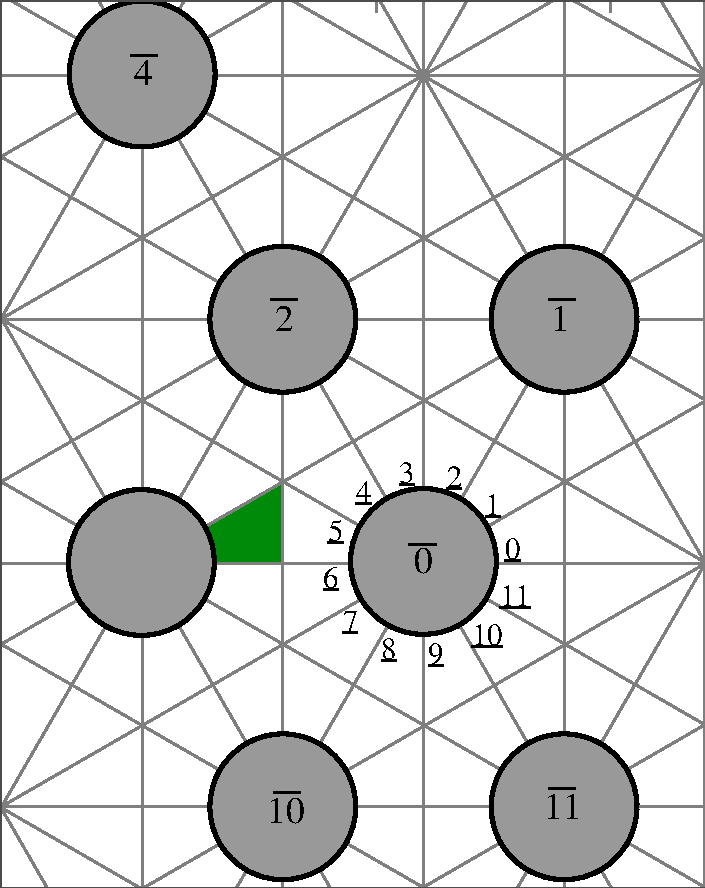
\includegraphics[width=0.35\textwidth]{diffuseFDSymbolIllustration}
  (b)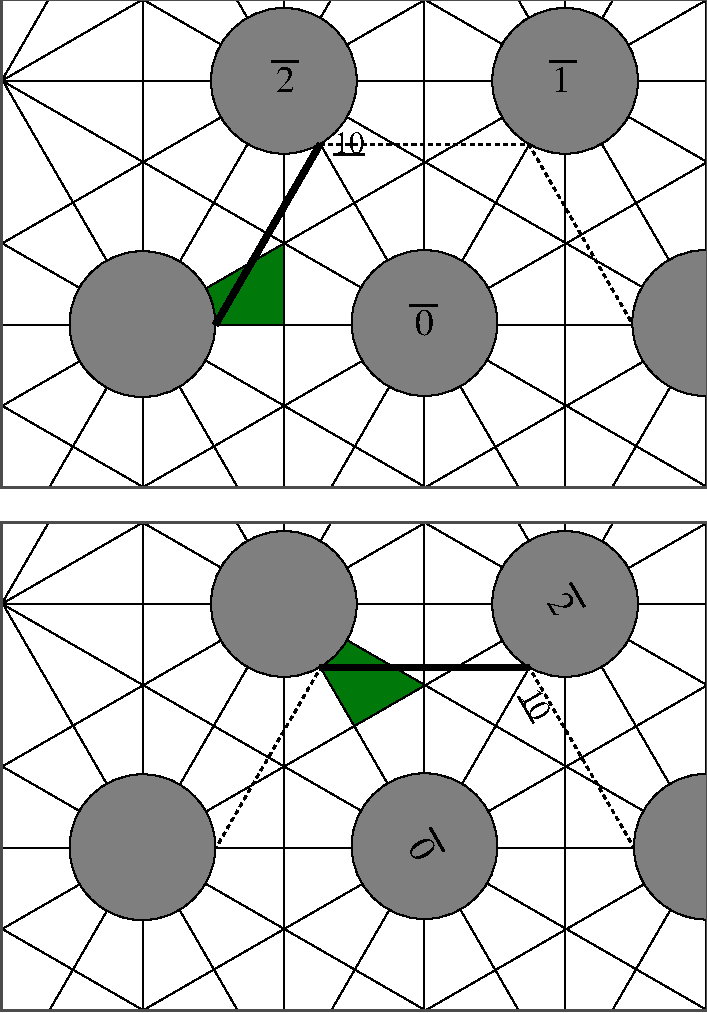
\includegraphics[width=0.35\textwidth]{diffuseFDSymbolOrbits}
  \caption{\label{fig-fdflights}
  Fundamental domain symbolic dynamics.
  (a) With  imposed finite horizon and starting on the edge of a disk in
  fundamental  domain (the green filled region), there are at most 6
  disks can be reached  without collision (disk
  $\overline{0},\overline{1},\overline{2},\overline{4},\overline{10}$ and
  $\overline{11}$). Similar to how elementary cell symbolic dynamics are
  created, we label the 12 triangular pieces of a disk in a counter
  clock-wise  manner, from $\underline{0}$ to $\underline{11}$. The
  combination of a disk  label and a triangular piece label
  $\{\overline{i},\underline{j}\}$ uniquely  identifies a topologically
  distinct flight.
  (b) The fundamental domain fixed point
  $\{\overline{2},\underline{10}\}$, which corresponds to a periodic
  orbit of length 6 in elementary cell ($\cycle{0246810}$), is unwrapped
  in   global space. After each collision we re-label the disks and
  triangular   partitions according to their relative positions to the
  ``new'' fundamental   domain. In the figure labels are also rotated
  according to the point   group actions.
  }
\end{figure}



In the international crystallographic notation, the hexagonal lattice is
called $p6mm$, with point group $6mm$, where prefix $p$ indicates that
the unit cell is primitive (not centered),
\beq
\Group = \{
e, C_6^+, C_6^-, C_3^+, C_3^-, C_2,
\sigma_{d1}, \sigma_{d2}, \sigma_{d3},
\sigma_{v1},\sigma_{v2}, \sigma_{v3}
\}
\,,
\eeq
with $s=\sigma_{d}$ the reflection across the short disk-disk separation,
and $\ell=\sigma_{v}$ reflection across the long disk-disk separation
generators of \Dn{12}. The entire space group $p6mm$is then generated by
adding a disk-to-disk generator $f$ that pivots a disk center to another
by flip across the symmetry line normal to the short disk-disk
separation, \reffig{fig-7diskFundDflips}a. We find it convenient to
define $C$ as the generator of cyclic rotations by $\pi/3$,
\beq
\ell s = C_6^- = C
\,,\quad
C^6 = e
\,;\qquad
s \ell =  C_6^+
\,,\qquad
s  =  C_6^+ \ell
\,.
\eeq
    \TZ{2015-10-22}
    {The idea is that the topological periodic orbit in the fundamental
    domain is not sensitive to the order of flips. When $w$ increases,
    one might notice that a single flight along the orbit changes from
    $sf$ to $fs$. However, the relative position between the start and
    end triangular cells are always the same.}
A free flight between two disks in the full space may then be wrapped
into fundamental domain, according to the sequence cell edges
$\{s,\ell,f\}$ it passed. For example, there are different paths when
jump to disk $0$: it can be as simple as a single pivot about $f$, or can
be more complex such like $\ell f s$ that involves multiple flips,
~\reffig{fig-7diskFundDflips} b. Although we can associate each free
flight with a chain of the generators, some of the combinations are
equivalent. The short jump $sf$ is topologically equivalent to $fs$, in
the sense that the particle ends up in the same copy of fundamental
domain before next collision.

Our task is to generate all distinct itineraries from $\{s,\ell,f\}$. One
can immediately realize a partial list of the equivalence relations:
\bea
f s &=& s f
\,,\nonumber\\
f \ell f&=&\ell f \ell
\,.
\eea
All longer equivalence relations in ~\reffig{fig-7diskFundDflips} can be
reduced to the above primitive ones:
\bea
f s \ell &=& s f \ell\,,\nonumber\\
\ell f\ell s &=& f \ell s f\,.
\eea

There are also some pruning rules to keep in mind. Because a free flight
cannot cross the same border twice, sequences including $\ell\ell,ff,ss$
are forbidden. $C^3$ (and all higher orders) is also pruned as the
particle cannot cross the center hard disk; nor swirl around it.

While the string description of flight is mathematically rigorous and
accurate, it is practically hard to be encoded into programs for
computing the orbits, because the number of equivalent strings increases
exponentially when the length (of a single string) increases. However,
there is a more physically intuitive way to organize the type of flight,
by means of ``topological flight'', \reffig{fig-fdflights} (a). In this
representation, a equivalence relation like $sf\equiv fs$ can be uniquely
identified by a combination of a disk number and a partition number
$\{\overline{0},\underline{6}\}$. Longer flight such like $\ell f \ell s
\ell f \equiv  f \ell f s \ell f \equiv f \ell s f \ell f \equiv f \ell s
\ell f \ell$ that cross many boundaries now yields a very simple symbol
pair $\{\overline{1},\underline{5}\}$.

The topological flight leads to a straight forward numerical scheme to
find cycles. The disk number fixes the two ends of the free flight while
the partition number limits the range of angles on the disk. Similar to
searching cycles in elementary cell, we now have a constrained version of
numerical minimization problem which can be solved using standard
non-linear optimization approach.
 \TZ{2015-11-02}
    {I have not yet talked about the pruning rule in detail here; it is
    more complicated bases on the reflection angle}

\subsection{Diffusion in the fundamental domain}
\begin{table}[htbp]
\hfill
\TZ{2015-10-19}{Do we need this many digits in the table?}
\begin{tabular}{|r|r|r|l|l|}
\hline
$\period{p}$ & \# cycles & $\zeta$(0,0) & $\lambda$ & D \\ \hline\hline
1      & 5      & -0.2169759 & 1.39193 & 0.37795 \\
2      & 10     & -0.0248233 & 1.74541 & 0.23118\\
3      & 33     & -0.0221962 & 1.72235 & 0.25257\\
4      & 108    & -0.0002192 & 1.74450 & 0.24165\\
5      & 373    &  0.0023463 & 1.76079 & 0.24468\\
6      & 1378   &  0.0096330 & 1.75610 & 0.24068\\ \hline\hline
\multicolumn{3}{|l|}{numerical experiment}
                           & 1.760 & 0.25
\\ \hline
\end{tabular}

\caption{\label{TCELL2}
  Results for $w$=0.3. Calculation in FD. Gaspard 1992
  note: ``My numerical estimate for the Lyapunov exponent when $w=0.3$ is
  $\lambda = 1.760 \pm 0.002$, which supports the result of this table.''
}
\end{table}

\begin{figure}[htbp]
  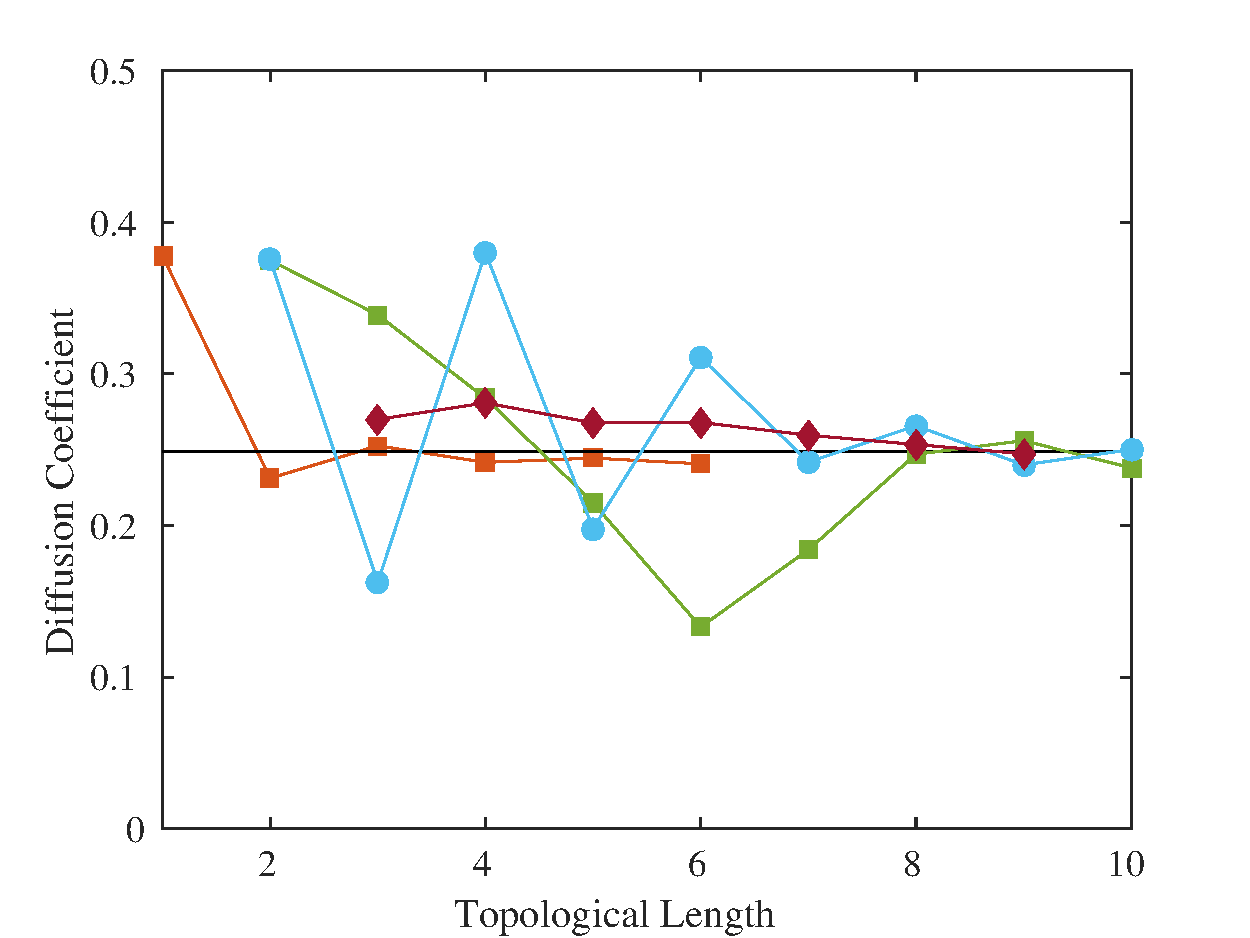
\includegraphics[width=0.45\textwidth]{diffuseCycleExpansionResults}
  \caption[]{\label{fig-convergence}
  The convergence of diffusion coefficients  calculated using cycle
  expansion in elementary cell (green squares),  fundamental
  domain(orange squares). We  also show the convergence of ``periodic
  orbit expansion'' method, with and  without Shanks transformation
  (circles and diamonds) discussed in  \refref{Morriss1994}. Here $w = 0.3$.
  }
\end{figure}

\begin{figure}
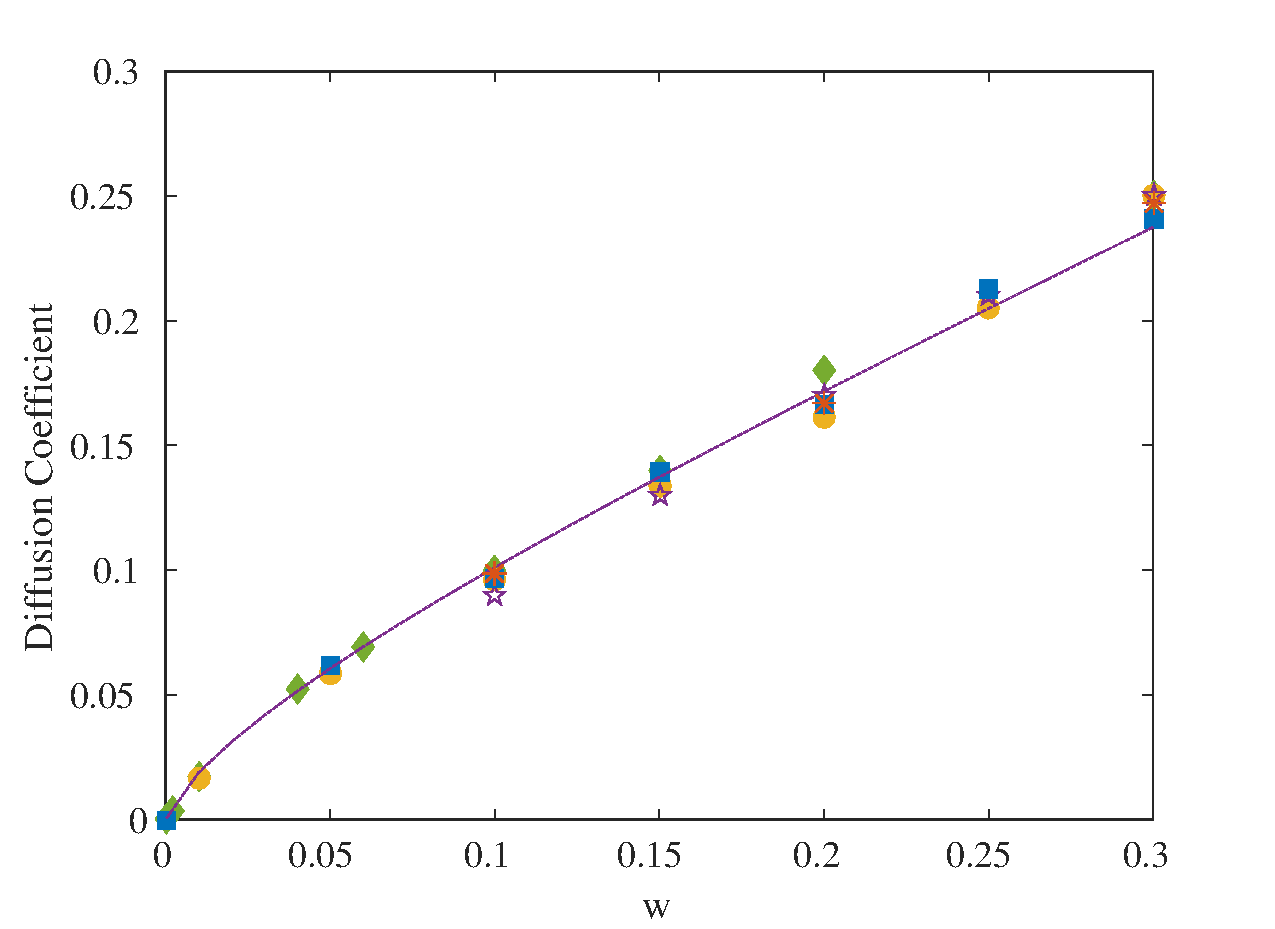
\includegraphics[width=0.45\textwidth]{diffuseDiffCoefPlot}
  \caption[]{\label{fig-results} Diffusion coefficients as a function $w$.  Figure generated using data from various resources. Diamonds are results from  Green-Kubo numerical experiments\rf{MacZwa83}; stars\rf{BaEvCo93} and  circles\rf{GasBar95} are calculated from escape rate; and triangles are  given by Hausdorff fractal dimension calculation\rf{GasBar95}; dashed line  is a statistical approximation\rf{Angstmann20121819}}.
\end{figure}

       \TZ{2015-10-19}{Any comment on caption of \reffig{fig-convergence}?}
Compared with various methods, the symmetry reduced cycle expansion
method converges the fastest, table \ref{TCELL2} and
\reffig{fig-convergence}. Diffusion coefficient computed from $\sim2000$
fundamental domain cycles of topological length up to 6 gives two
significant digits, while the elementary cell calculation needs over
$\sim 10000$ cycles in order to converge. In other words, the fundamental
domain cycles suggests a better and denser partition of the phase space.
    \TZ{2015-10-19}{Talk about other two methods}.

To further test \refeq{eq-meanSquareDisp}, we compute the diffusion
coefficient for $w/r = 0.05, 0.10, 0.15, 0.20, 0.25, 0.30$, and compare
the results with existing numerical experiments and a recent statistical
estimation, \reffig{fig-results}. In Green-Kubol velocity
auto-correlation method the  diffusion coefficient can be extrapolated to
the accurate reference value $0.250$ (at $w/r=0.30$), using ensembles of
$10^6\sim10^7$ gas particles flying for long time $T>20$ (and the number
of bounces is greater than this)\rf{MacZwa83}. On the other hand, while
statistical approach yields a smooth analytical
formula\rf{Angstmann20121819}, the diffusion property is fundamentally
never a smooth, monotonically increasing function of $w$
    \TZ{2015-11-02}
    {what is that 1D diffusion reference that shows the anywhere
    continuous, nowhere smooth curve?}
Again, the effectiveness (yet correctness) of the cycle expansion is
proved by those comparison.

\section{Conclusion}

 \TZ{2015-11-02}{What else do we put here?}
% Specify following sections are appendices. Use \appendix* if there
% only one appendix.
%\appendix
%\section{}

\begin{acknowledgments}
We are grateful to Pavel M. Svetlichnyy for many fruitful discussions in
the early stages of this project, and the key suggestion that the plane
can be tiled in terms of three elementary tiling generators.
TZ was supported by NSF grant ???-?????.
PC thanks to the family of late G. Robinson, Jr. and NSF grant
DMS-1211827 for partial financial support.
\end{acknowledgments}

\ifboyscout
% switch to Private
\newpage
    % reducesymm/tingnan/flotsam.tex    master file: diffuse/main.tex

\section{ZhCvGo15 flotsam}
\label{s:flotsam}

Squirrel away here potentially recyclable text from the
paper\rf{ZhCvGo15} proper, \texttt{diffuse/ZhCvGo15.tex}

%remember to cite Cvitanovi\'c and Eckhardt\rf{CvitaEckardt} {\em Symmetry
%decomposition of chaotic dynamics}

%A test of hyperlinking: what looks better?
%
%DasBuch\rf{DasBuch}
%or
%\refref{DasBuchMirror} {Chapter ``{World} in a mirror''}
%or trace~\refref{CBtrace}
%or \refref{Froeh10}
%or ChaosBook convergence\rf{CBconverg}
%or Predrag\rf{Cvi07}

As a billiard built up completely of concave surfaces and as a pure
hyperbolic system, the Lorentz gas is a good candidate for description in
terms of cycle expansions\rf{AACI}.

                                                            \toCB
\refRef{solomon1994chaotic} {\em Chaotic advection in a two-dimensional
flow: L\'evy flights and anomalous diffusion} studies chaotic transport
experimentally passive tracers in $2$\dmn\ rotating in laminar, chaotic,
and turbulent flows which can be described as anomolous deterministic
diffusion in periodic arrays. We do not touch that here.


%
%%%%%%%%%%%%%%%%%%%%%%%%%%%%%%%%%%%%%%%%%%%%%%%%%%%%%%%%%%%%%%%%%%
%\SFIG{fig_lor_4}
%{}{
%Deterministic diffusion in a
%finite horizon periodic Lorentz gas.
%\hfill (T. Schreiber)
%}{fig-lor-4}
%%%%%%%%%%%%%%%%%%%%%%%%%%%%%%%%%%%%%%%%%%%%%%%%%%%%%%%%%%%%%%%%%%
%

As a gedanken experiment, suppose a passively controlled robot is moving
in a boulder field at constant speed. The diffusion coefficient, which
describes roughly how much area the robot explored in a unit time, is the
key quantity we would like to investigate. We place the boulder in a
regular, periodic array and assume that we are in the heavy boulder limit
such that after each collision event, only the robot is deflected and
boulders remain immobilized. With the presumptions we effectively created
a periodic Lorentz gas model\rf{Dettm14} for locomotion in a boulder
field.

In biological field,  many important dynamical processes (often at
cellular level) are described in  terms of diffusion coefficients. Such
examples include the transport of ions  across the cell
membranes\rf{Stein12} and the movement of  microorganism(e.g.
bacterials) through natural  ecosystems\rf{koch1990diffusion}. In this
paper we will discuss the transport  property of more "macroscopic"
systems (such as moving  robots\rf{saranli2001rhex}) where a ``diffusive
description'' also applies.

Chaotic motions exist in many field of physics systems, blah. There are
physical problems such as beam defocusing in particle accelerators or
chaotic behavior of passive tracers in $2$\dmn\ rotating flows which can
be described as deterministic diffusion in periodic arrays. In the field
of animal/robotic locomotion, we will show that a macroscopic ``diffusion
view'' also applies.

In the macroscopic world, there are recent
studies shown that robotic locomotion in heterogeneous granular
environment also demonstrates scattering-diffusive pattern.

Lately, there has been an increased focus on robot locomotion in complex
environments (check Science and ROPP reference, the systematic study of
interactions between environment and locomotion, which we now
call``robophysics''). Many of those studies use substrates that are
spatially homogeneous and we have a good
understanding\rf{li2009sensitive,li2013terradynamics}. However, little is
known for locomotion in heterogeneous environment. There are some limited
experimental/theoretical studies for relatively simple settings (e.g.
slopes,ref). In this paper we intend to approach the longterm transport
properties of locomotion in a more complex environment, i.e. in a field
of scatterers of which the scales are comparable to the locomotor.


 As we are concerned with the long time behavior,
 this problem can be circumvented
 by replacing $ \hf^t(\tx{\tpk}) $ by the mean
 drift in the $t \rightarrow \infty$ limit.
 $ \hf^t(\tx{\tpk}) $ is a translation in $\hM$ for each
 complete cycle $p$ in $M$, so we replace
 \bea
 \hf^t(\tx{\tpk}) - \tx{\tpk}
 \,\Longrightarrow \,
 &&
 { { \hf^{m_p t}(\tx{\tpk}) - \tx{\tpk} }
 % \over         m_p
 }
    % \,\equiv \, r {\tilde n}_{\tp} (\tx{\tpk})
 \continue
t &=& r \period{\tilde{p}}, \quad m_p = \period{p}/\period{\tilde{p}} \quad \tx \in \tp \,\, ,
 \eea
 in Eq.~(240).
 The magnitude of ${\tilde n}_{\tp}(\tx{\tpk})$, the mean
 global drift per one traversal of the fundamental cycle $\tp$, is
 independent of the starting point, but its direction is not; the
 reason is that each fundamental domain cycle corresponds to a set of
 trajectories in $\hM$.
 The ${1 \over {|G|}} \sum$ average in
 Eq.~(240) then generates all distinct global drift
 directions, so we can again replace the
 sum over cycle points by the factor $\period{\tilde{p}}$, and obtain the
 $Z$ function Eq.~(14) for the $\alpha $ irreducible subspace
 $$
 Z(\beta,s)_\alpha\,=\,\prod_{\tp \in \t{\cal{P}} } \exp
 % \left( -
  % \sum_{r=1}^\infty {1 \over r}
 % {{
  % \chi_\alpha(h^r_{\tp})
  % }
 % \over
 % { | \det \left( \bf{1}-\t{\bf J}_{\tp}^{r} \right) | }
 % }
 % e^{ ( \beta \cdot {\tilde n}_{\tp} - s \period{\tilde{p}}) r}
  % \right)
 \,\, .
 Eq.~(24)
 $$
 $\hn_{\period{\tilde{p}}}(\tx_k)$
%{\tt NOnsense...}
 The leading eigenvalue of the
unsymmetrized
 operator Eq.~(8) is
 the leading eigenvalue of the symmetric subspace for which
 $\chi_\alpha(g)=1$ for all $g \in G$.

The interesting dynamical averages is determined by the spectrum of the operator
\beq \det(\eigenvL - \Lop) \,=\,\prod_{p} \exp \left(
  - { \sum_{r=1}^\infty {1 \over r} { e^{(\beta \cdot \hn_p- s
        \period{p}) r} \over \oneMinJ{r} }
  } \right) \,,
\ee{lor-diff-14}
or the corresponding \dzeta\
% \newpage
\fi


% Choosing a journal automatically selects the correct APS BibTeX style
% file (bst file), so only uncomment the line below if necessary.
% \bibliographystyle{apsrev4-1}
\bibliography{../bibtex/siminos,../bibtex/diffuse}


\end{document}



% If in two-column mode, this environment will change to single-column
% format so that long equations can be displayed. Use sparingly.
% \begin{widetext}
%   put long equation here
% \end{widetext}

% Use the figure* environment if the figure should span
% across the entire page. There is no need to do explicit centering.

% Surround figure environment with turnpage environment for landscape
% figure
% \begin{turnpage}
%   \begin{figure}
%     \includegraphics{}%
%     \caption{\label{}}
%   \end{figure}
% \end{turnpage}

% Here is an example of the general form of a table:
% Insert the column specifiers (l, r, c, d, etc.) in the empty braces of the
% \begin{tabular}{} command.  The ruledtabular enviroment adds doubled
%   rules to table and sets a reasonable default table settings.  Use
%   the table* environment to get a full-width table in two-column Add
%   \usepackage{longtable} and the longtable (or longtable*}
%   environment for nicely formatted long tables. Or use the the [H]
%   placement option to break a long table (with less control than in
%   longtable).
% \begin{table}%[H] add [H] placement to break table across pages
% \caption{\label{}}
% \begin{ruledtabular}
%   \begin{tabular}{}
% Lines of table here ending with \\
% \end{tabular}
% \end{ruledtabular}
% \end{table}

% Surround table environment with turnpage environment for landscape
% table
% \begin{turnpage}
%   \begin{table}
% \caption{\label{}}
% \begin{ruledtabular}
%   \begin{tabular}{}
% \end{tabular}
% \end{ruledtabular}
% \end{table}
% \end{turnpage}
